\documentclass[aa]{lib/aa}
\bibpunct{(}{)}{;}{a}{}{,} % to follow the A&A style
\usepackage{graphicx}
\usepackage{comment}
\usepackage{txfonts}
\usepackage{stfloats}
%\usepackage{algorithm}
%\usepackage{algpseudocode}
\newcommand{\spz}[1] {{\texttt{\textbf{SPZ: #1}}} }
\newcommand{\eh}[1] {{\texttt{\textbf{ EH: #1}}} }
\newcommand{\LSun}{\mbox{${L}_\odot$}}
\newcommand{\MSun}{\mbox{${M}_\odot$}}
\newcommand{\Msun}{\mbox{${M}_\odot$}}
\newcommand{\RSun}{\mbox{${R}_\odot$}}
\newcommand{\MJup}{\mbox{${M}_{\rm Jup}$}}

\def\apgt{\ {\raise-.5ex\hbox{$\buildrel>\over\sim$}}\ }
\def\aplt{\ {\raise-.5ex\hbox{$\buildrel<\over\sim$}}\ }
\def\lteq{\ {\raise-.5ex\hbox{$\buildrel<\over-$}}\ }

\newcommand{\jumbo}{\mbox{JuMBO}}
\newcommand{\jumbos}{\mbox{JuMBOs}}

%\algnewcommand{\LineComment}[1]{\State \(\triangleright\) #1}
%\def\ind#1#2{\hbox{\hskip 0.0truein\hbox to 0.2truein{#1\hfil}
%	        \hbox{\hsize 6.0truein\vtop{\ni#2}\hfil}}\vskip 1pt}

%-----------------------------------------------------------------------

\begin{document} 

   \title{The primoridal origin of Jupiter mass Binary Objects}
%   \author{E. Hochart\inst{1}
%          \and
%          S. Portegies Zwart\inst{1}
%          }
   \institute{
             Leiden Observatory, University of Leiden, 
             Niels Bohrweg 2, 2333 CA Leiden\\
             \email{hochart@mail.strw.leidenuniv.nl}
             \email{spzstrw.leidenuniv.nl}
             }
   \date{Received XXXXX; accepted XXXXXX}

%--------------------------------------------------------------------
  \abstract
  %% context heading (optional)
      {The recently observed population of 540
  free-floating jupiter-mass objects, and 42 dynamically soft pairs of
  jupiter-mass planets, among which 2 with a tertiary companion, in the Trapezium cluster has
  raised interesting questions on their formation and further
  evolution. }
  % aims heading
   {We test various scenarios for the origin and survivability of
  these free floating jupiter-mass planets and Jupiter-mass Binary Objects
  (JuMBOs) in the Trapezium cluster.  }
   % methods heading
   {The numerical calculations are performed by direct N-body
     integration of the stars and planets in the Trapezium cluster
     starting with a wide variety of planets in various
     configurations. We discuss four main models: $\mathcal{SPP}$ in
     which selected stars have two outer orbiting jupiter-mass
     planets; $\mathcal{SPM}$ where selected stars are orbited by 
     jupiter-mass planet-moon pairs; $\mathcal{ISF}$ in which
     \jumbos\, are formed in situ together with the stars. and
     $\mathcal{FFC}$ where we introduce a large population of free
     floating single jupiter-mass objects, but no binaries.  }
   % results heading
   {Models $\mathcal{SPP}$ and $\mathcal{FFC}$ spectacularly fail to
     produce enough \jumbos. Models $\mathcal{SPM}$ can produce
     sufficient free floaters and \jumbos\, but require to start with
     unrealistically wide orbits for the planet-moon system around the
     star.  The observations are best explained with in situ formation
     (model $\mathcal{ISF}$) of \jumbos.  }
   % conclusions heading (optional)
   {The observed populations of \jumbos\, and free floating planets in
     the Trapezium cluster are best reproduced if all planets formed in
     pairs together with the other stars in a fractal distribution
     with a virial radius of $\sim 0.5$\,pc.  }
   
   \keywords{...}

   \maketitle
   
%-------------------------------------------------------------------
\section{Introduction}

Recently \cite{2023arXiv231001231P} reported on the discovery of 42
Jupiter-Mass Binary Objects (\jumbos) in the direction of the
Trapezium cluster.  Their component masses range between 0.6\,\MJup\,
and 14\,\MJup\, and have projected separations between 25\,au and
380\,au.  Two of these objects have a nearby tertiary jupiter-mass
companion.  They also observed a population of 540 single objects in
the same mass range. This discovery initiates the discussions on the
origin and surviveability of weakly bound jupiter-mass pairs in a
clustered environment.

The first single free-floating jupiter-mass objects have been found in
the direction of the Trapzium cluster more than 20 years ago
\citep{2000Sci...290..103Z,2000MNRAS.314..858L,2000AGM....17..A11M}.
Many more have been found since then, for example in the young
clustered environment of Upper Scorpio \citep{2022NatAs...6...89M}, and
through gravitational microlensing surveys in the direction of the
Galactic bulge \citep{2011Natur.473..349S}.  Their abundance may be as
high as $1.9^{+1.3}_{-0.8}$ per star \citep{2011Natur.473..349S},
although a considerable fraction of these could be in wide orbits.

The origin of free floating planets has been actively debated. Star
formation, from the collapse of a molecular cloud through
gravitational instability, generally is expected to lead to objects
considerably more massive than Jupiter
\citep{1976MNRAS.176..367L,2005A&A...430.1059B}.  As a consequence,
the large population of jupiter-mass free-floaters is considered to
result from fully packed planetary systems, or kicked out of their
orbit by encounters with other stars in the young cluster. Single
jupiter-mass free floating objects then originally formed in a disk
around a star but became single later in life
\citep{1996Sci...274..954R,2015MNRAS.453.2759Z,2002ApJ...565.1251H,2017MNRAS.470.4337C,
  2019MNRAS.489.2280F, 2019A&A...624A.120V}.  The number of
super-jupiter mass free floating planets formed in this way is
expected to be on the order of one ($\sim 0.71$) per star
\citep{2019A&A...624A.120V}, but lower-mass free floaters orphaned
this way may be much more abundant \citep{2002ApJ...565.1251H}.  The
origin of relatively massive free-floaters through dynamical phenomena
is further complicated by the tendency for lower mass planets to be
more prone to ejections
\citep{2001Icar..150..303F,2013MNRAS.433..867H,2019MNRAS.489.2280F,2020MNRAS.497.1807S}.

Explaining the observed abundance and mass-function of single
free-floating jupiter-mass objects appears to be difficult, but
recently a new population of paired free floaters have been
discovered.  So far, binary object have been discovered in tight (few
au) orbits \citep{2021ApJS..253....7K}.  Known interstellar
jupiter-mass binary objects include only four objects:
\begin{itemize}
\item[$\bullet$]2MASS J11193254-1137466 AB: a $5$ to 10\,\MJup\,
  primary in a $a=3.6\pm0.9$\,au orbit \citep{2017ApJ...843L...4B}.
\item[$\bullet$]WISE 1828+2650: a 3 to 6\MJup\, primary with a
  5\,\MJup\ companion in an $\apgt 0.5$\,au orbit
  \citep{2013ApJ...764..101B}.
\item[$\bullet$] WISE J0336-014: a $8.5$ to
  $18$\,\MJup\ primary with a $5$ to $11.5$\,\MJup\, companion in a
  $0.9^{+0.05}_{-0.09}$\,au orbit \citep{2023ApJ...947L..30C}.
\item[$\bullet$]2MASS J0013-1143 discovered by \citep{2017AJ....154..112K} and
  suspected to be a binary by \citep{2019A&A...629A.145E}.
\end{itemize}

Such tight pairs could have formed as binary planet or a planet-moon
pairs which are dislodged from their parent star to become \jumbos\,
\citep{2016ApJ...819..125C}.  However, since only a few were
discovered such an exotic scenario seems to pose a reasonable
explanation for their existence.  The new discovery of a rich
population of $42$ wide (25\,au to 380\,au) \jumbos\,
\citep{2023arXiv231001231P} requires a more thorough study on their
origin.

Adopting a dynamical origin, or at least a dynamical history, we
perform direct N-body simulations of a Trapezium-like cluster with
primordial planets and \jumbos. With the simulations, we focus on four
models that could explain the abundance and orbital characteristics of
the observed jupiter-mass objects (JMO) in the cluster. In this paper,
we perform a rudimentary analysis on four scenarios capable of forming
\jumbos.  Alternative to forming in situ (scenario ${\cal ISF}$, from
in-situ formation), one can naively imagine three mechanisms to form
\jumbos. \citep{2023arXiv231006016W} argued that these binaries could
be explained from planetary systems of which the outer two planets are
stripped by a passing star in a close encounter. The two ejected
planets would lead to a population of free floating planets, but could
also explain the observed population of \jumbos.  We call this
scenario ${\cal SPP}$ (for star planet-planet).

Alternatively one could imagine \jumbos\, to result from planet-moon
pairs orbiting some star that is ejected to become a \jumbo.  We call
this scenario ${\cal SPM}$, for star planet-moon.

Finally, one could imagine that a sufficiently large population of
free-floating jupiter-mass objects could lead to a population of
\jumbos\,by dynamical capture of one JMO by another.  We call this
scenario ${\cal FFC}$ (free floating capture). A similar scenario was
proposed by \citep{2010MNRAS.404.1835K} for explaining very wide
stellar pairs, but the model was also adopted to account for wide
planetary orbits \citep{2012ApJ...750...83P,2018MNRAS.473.1589G}

We start by discussing some fundamental properties of the
environmental dynamics, followed by a description of numerical
simulations to characterize the parameters of the acquired \jumbos\, and
the resulting occurrence rates. 

%--------------------------------------------------------------------
\section{The dynamical characterization of \jumbos}

The \jumbos\, discovered by \citep{2023arXiv231001231P} were located
in the Trapezium cluster. We base our analysis on the parameters
derived for this cluster by \citep{2016MNRAS.457..313P} by numerical
modeling of disk-size distributions observed in the Trapezium cluster,
and concluded that this distribution is best reproduced for a cluster
containing $\sim 2500$ stars with a total mass of $\sim 900$\,\MSun\,
and a half-mass radius of $\sim 0.5$\,pc. The results were only
consistent with the observations if the initial cluster density
distribution represented a fractal dimension of 1.6, and was
inconsistent with a \citep{1911MNRAS..71..460P} distribution.
Nevertheless, for consistency with earlier studies, we perform our
analysis for Plummer as well as for a fractal (with fractal dimension
1.6) distributions.

Adopting a Plummer distribution of the Trapezium cluster (with $r_{\rm
  vir} = 0.5$\,pc virial radius), the cluster core radius $r_c \simeq
0.64r_{\rm vir} \sim 0.32$\,pc with a core mass of 250\,\MSun. This
results in a velocity dispersion of $v_{\rm disp} \equiv
GM/\sqrt{r_c^2 + r_{\rm vir}^2} \simeq 0.97$\,km/s. With a mean
stellar mass in the cluster core of 1\,\MSun\, the unit of energy
expressed in the kinematic temperature kT becomes $\sim 8 \cdot
10^{42}$\,erg.

Jumbos are found in the mass range of about 0.6\,\MJup\, to
14\,\MJup\, and have a projected separation of 25\,au\, and $\sim
380$\,au.  The averaged observed values are $d=200\pm109$\,au,
$\langle M\rangle = 4.73\pm3.48$\,\MJup, and $\langle m\rangle =
2.81\pm2.29$\,\MJup. The median and 25\,\% to 75\,\% percentiles are
$d = 193.75^{+78.225}_{-114.075}$\,au $M =
3.67^{+1.31}_{-1.57}$\,\MJup, and $m = 2.10^{+1.05}_{-1.05}$\,\MJup.

To simplify our analysis, let us assume that the observed variation in
projected distances between the two Jupiter-mass objects corresponds
to an orbital separation and express distances in terms of semi-major
axis (see Appendix A for motivation).  In theory, the is a clear
difference between the projected separation and the actual semi-major
axis of the orbit, and this difference depends on the underlying
eccentricity distribution (which is not measured in the observed
\jumbos), but in practice this difference is negligible compared to
the 25\% to 75\% uncertainty intervals.

To first order, the binding energy of jumbos then ranges between $\sim
5\cdot 10^{37}$\,erg and $1.4\cdot 10^{41}$\,erg, or at most $\sim
0.02$\,kT. This makes them soft upon an encounter with a cluster star.

The hardest \jumbo, composed of two 14\,\MJup\, planets in a 25\,au
orbit would be hard for another encountering object of less then
$17\,M_{\rm Jupiter}$.  For an encountering 1\,\MJup\, object a 25\,au
orbit would be hard only if the two planets are about three times as
massive a Jupiter.  This entails that \jumbos\, are often soft for any
encountering free floating planet unless they are in tight enough
orbits or the perturber is of low mass.  On average, soft encounters
tend to soften these binaries even further
\citep{1975MNRAS.173..729H}, although an occasional soft encounter
with another planet may actually slightly harden the \jumbo.
Independent of how tight the orbit, \jumbos\, are expected to be
relatively short lived, because they dissociate upon a close encounter
with any other cluster member.  Once ionized they contribute to the
population of free floating single objects.  Note that in the
Trapezium cluster, the orbits of 2MASS J11193254-1137466AB, WISE
1828+2650, and WISE J0336-014 would be hard; they could therefore be
the fittest survivors of an underlying population.

To further understand the dynamics of the jumbos in a clustered
environment, and to study the efficiency of the various formation
scenarios we perform $N$-body calculations of the Trapezium star
cluster with a population of jupiter-mass objects in various initial
configurations.

%--------------------------------------------------------------------
\section{Methodology}

For each of our proposed models, ${\cal ISF}$ (in situ formation of
jumbos), ${\cal SPP}$ (\jumbos\, formed via ejections of a host stars
outer planets), ${\cal SPM}$ (as planet-moon pairs orbiting a star),
and ${\cal FFC}$ (as mutual capture of free-floaters) we perform a
series of $N$-body simulations with properties consistent with the
Trapezium cluster.

Each cluster starts with 2500 single stars taken from a broken
power-law mass-function \citep{2002Sci...295...82K} between
0.08\,\MSun\, and $30$\,\MSun\, distributed either in a Plummer sphere
(model Pl) or a fractal distribution with a fractal dimension of 1.6
(model Fr). All models start in virial equilibrium.  We run three
models for each set of initial conditions, with a virial radius of
0.25\,pc, 0.5\,pc and 1.0\,pc, called model R025, R05 and R100,
respectively.  We ignore stellar evolution, as well as the tidal field
of the Galaxy. We further assume stellar radii to follow the zero-age
main sequence, and the radius of jupiter-mass objects based on a
density consistent with Jupiter.

For each of our proposed models, we initialize a population of single
or binary JMO. The single (and primaries in primordial \jumbos) are
selected from a power-law mass function between 0.8\,\MJup\, and
14\,\MJup, which is consistent with the observed mass function
\citep{2023arXiv231001231P}. We fitted a power-law to the
primary-planet mass function, which has a slope of $\alpha_{\jumbo}
=-1.2$ (considearbly flatter than Salpter's $\alpha_{\rm Salpter} =
-2.35$).  The first dozen discovered free floaters already seemd to
have a rather flat mass function \citep{2000MNRAS.314..858L}, but the
large statistics available through gravitational microlensing surveys
allowd a reliable estimate of the slope, which yields $\alpha =
-1.3^{+0.3}_{-0.4}$ \citep{2011Natur.473..349S}. This mass function is
somewhat steeper than the slope derived for lower-mass free floaters
($\alpha = -0.96^{+0.47}_{-0.27}$ \citep{2023AJ....166..108S}).

For the models with free-floating jupiter-mass objects, scenario
${\cal FFC}$, we sprinkle the single planets in the cluster potential
as single objects using the same initial distribution function as we
used for the single stars.  These models were run with
1200\,jupiter-mass objects (or 600 pairs), but we performed additional
runs with $10^3$ and $10^4$ free floaters.

Primordial \jumbos\, (model ${\cal ISF}$) are initialized with
semi-major axis with a flat distribution between 10\,au and $100$\,au
(in some cases $10^4$\,au), an eccentricity from the thermal
distribution between 0 and 1, and a mass ratio (also from the thermal
distribution) between 0.2 and 1.  The binary is subsequently rotated
to a random orientation. 

Isolated binaries, for scenario ${\cal ISF}$, are subsequently
sprinkled in the cluster potential as single objects using the same
initial distribution function as used for the single stars.

For scenario ${\cal SPM}$ we put the bound planet-moon pair in orbit
around a star.  The orbit of the planet-moon pair is circular and with
a random orientation at a distance from the star such that the
planet-moon's orbital separation is one-third of it's Hill radius.
This guarantees a stable planet-moon pair in orbit around the selected
star.

We selected the star to host such a planet-moon pair from 150 stars
lower in mass than 0.6\,\MSun\, and 150 more massive stars. The
mid-mass point (of 0.6\,\MSun) is almost twice the mean stellar mass
in the mass function.

For scenario ${\cal SPP}$, we select the same planet masses as for the
primordial \jumbos\, except that we have them orbiting one of the
selected stars as a hierarchical planetary system. The distance from
the first planet $a_1$ and the second planet $a_2$ (such that
$a_2>a_1$) are selected according to various criteria.  The inner
orbit $a_1$ was selected between 20\,au and $2000$\,au from a flat
distribution in $a$.  The outer orbit, $a_2$, we typically chose to be
ten times larger than the inner planet's Hill radius, but we also
perform simulations with five times and twice the Hill radius (we call
them model rH10, rH05 and rH02, respectively).

We perform an additional series of runs with pre-specified orbital
separations for the two planets $a_1$ and $a_2$, to follow the model
proposed in \citep{2023arXiv231006016W}.

Each run was repeated 10 times to deal with potential statistical
fluctuations, but we run 40 initiations of models ${\cal SPP}$\_Pl\_R025.

Each simulation is stopped at an age of 1\,Myr, after which we study
the population of free floating jupiter-mass objects and the
population of \jumbos.

To summarize, we performed the following model calculations:\\
\begin{tabular}{ll}
${\cal SPP}$ & As outer orbiting planets\\
${\cal SPM}$ & As bound planet-moon pair orbiting a star\\
${\cal FFC}$ & Free floating single planets.\\
${\cal ISF}$ & In situ formation of jumbos\\
\end{tabular}
In figure\,\ref{Fig:models} we illustrate the four models with a
schematic diagram.

%% \begin{figure}
%%     \centering
%% ${\cal SPP}$ 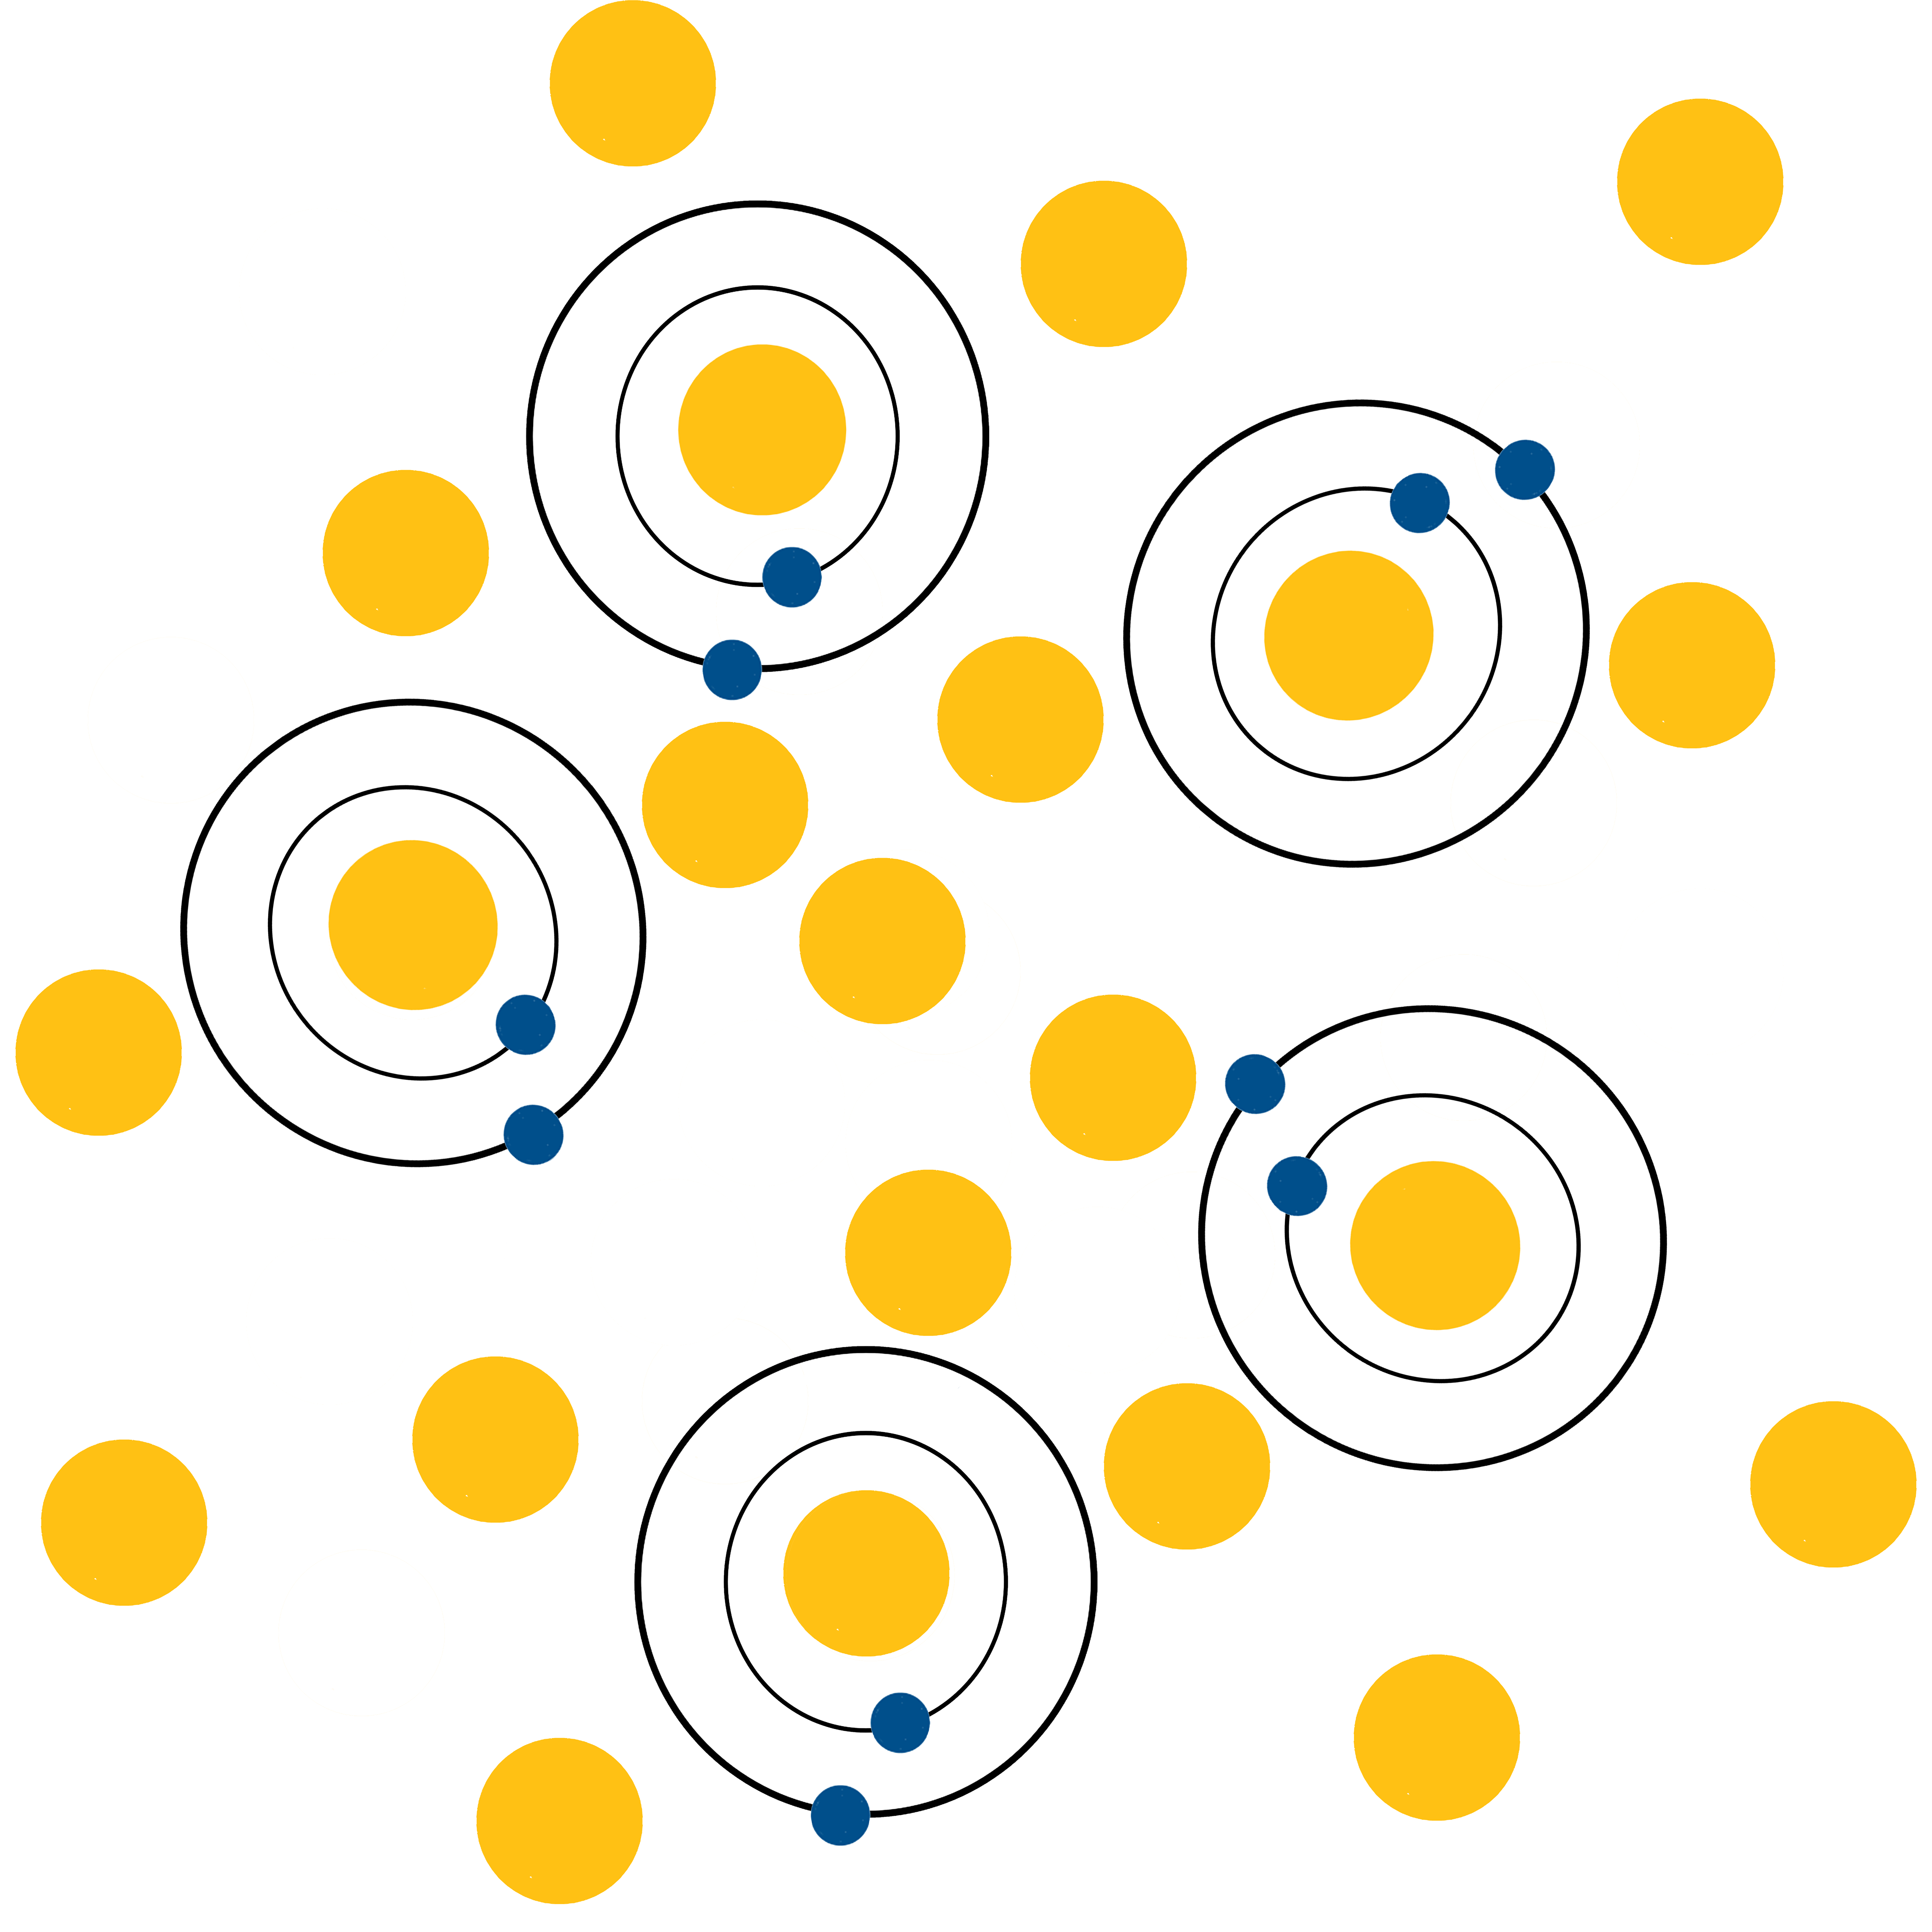
\includegraphics[width=.4\columnwidth]{figures/Model_PP.png}
%% ${\cal SPM}$ ~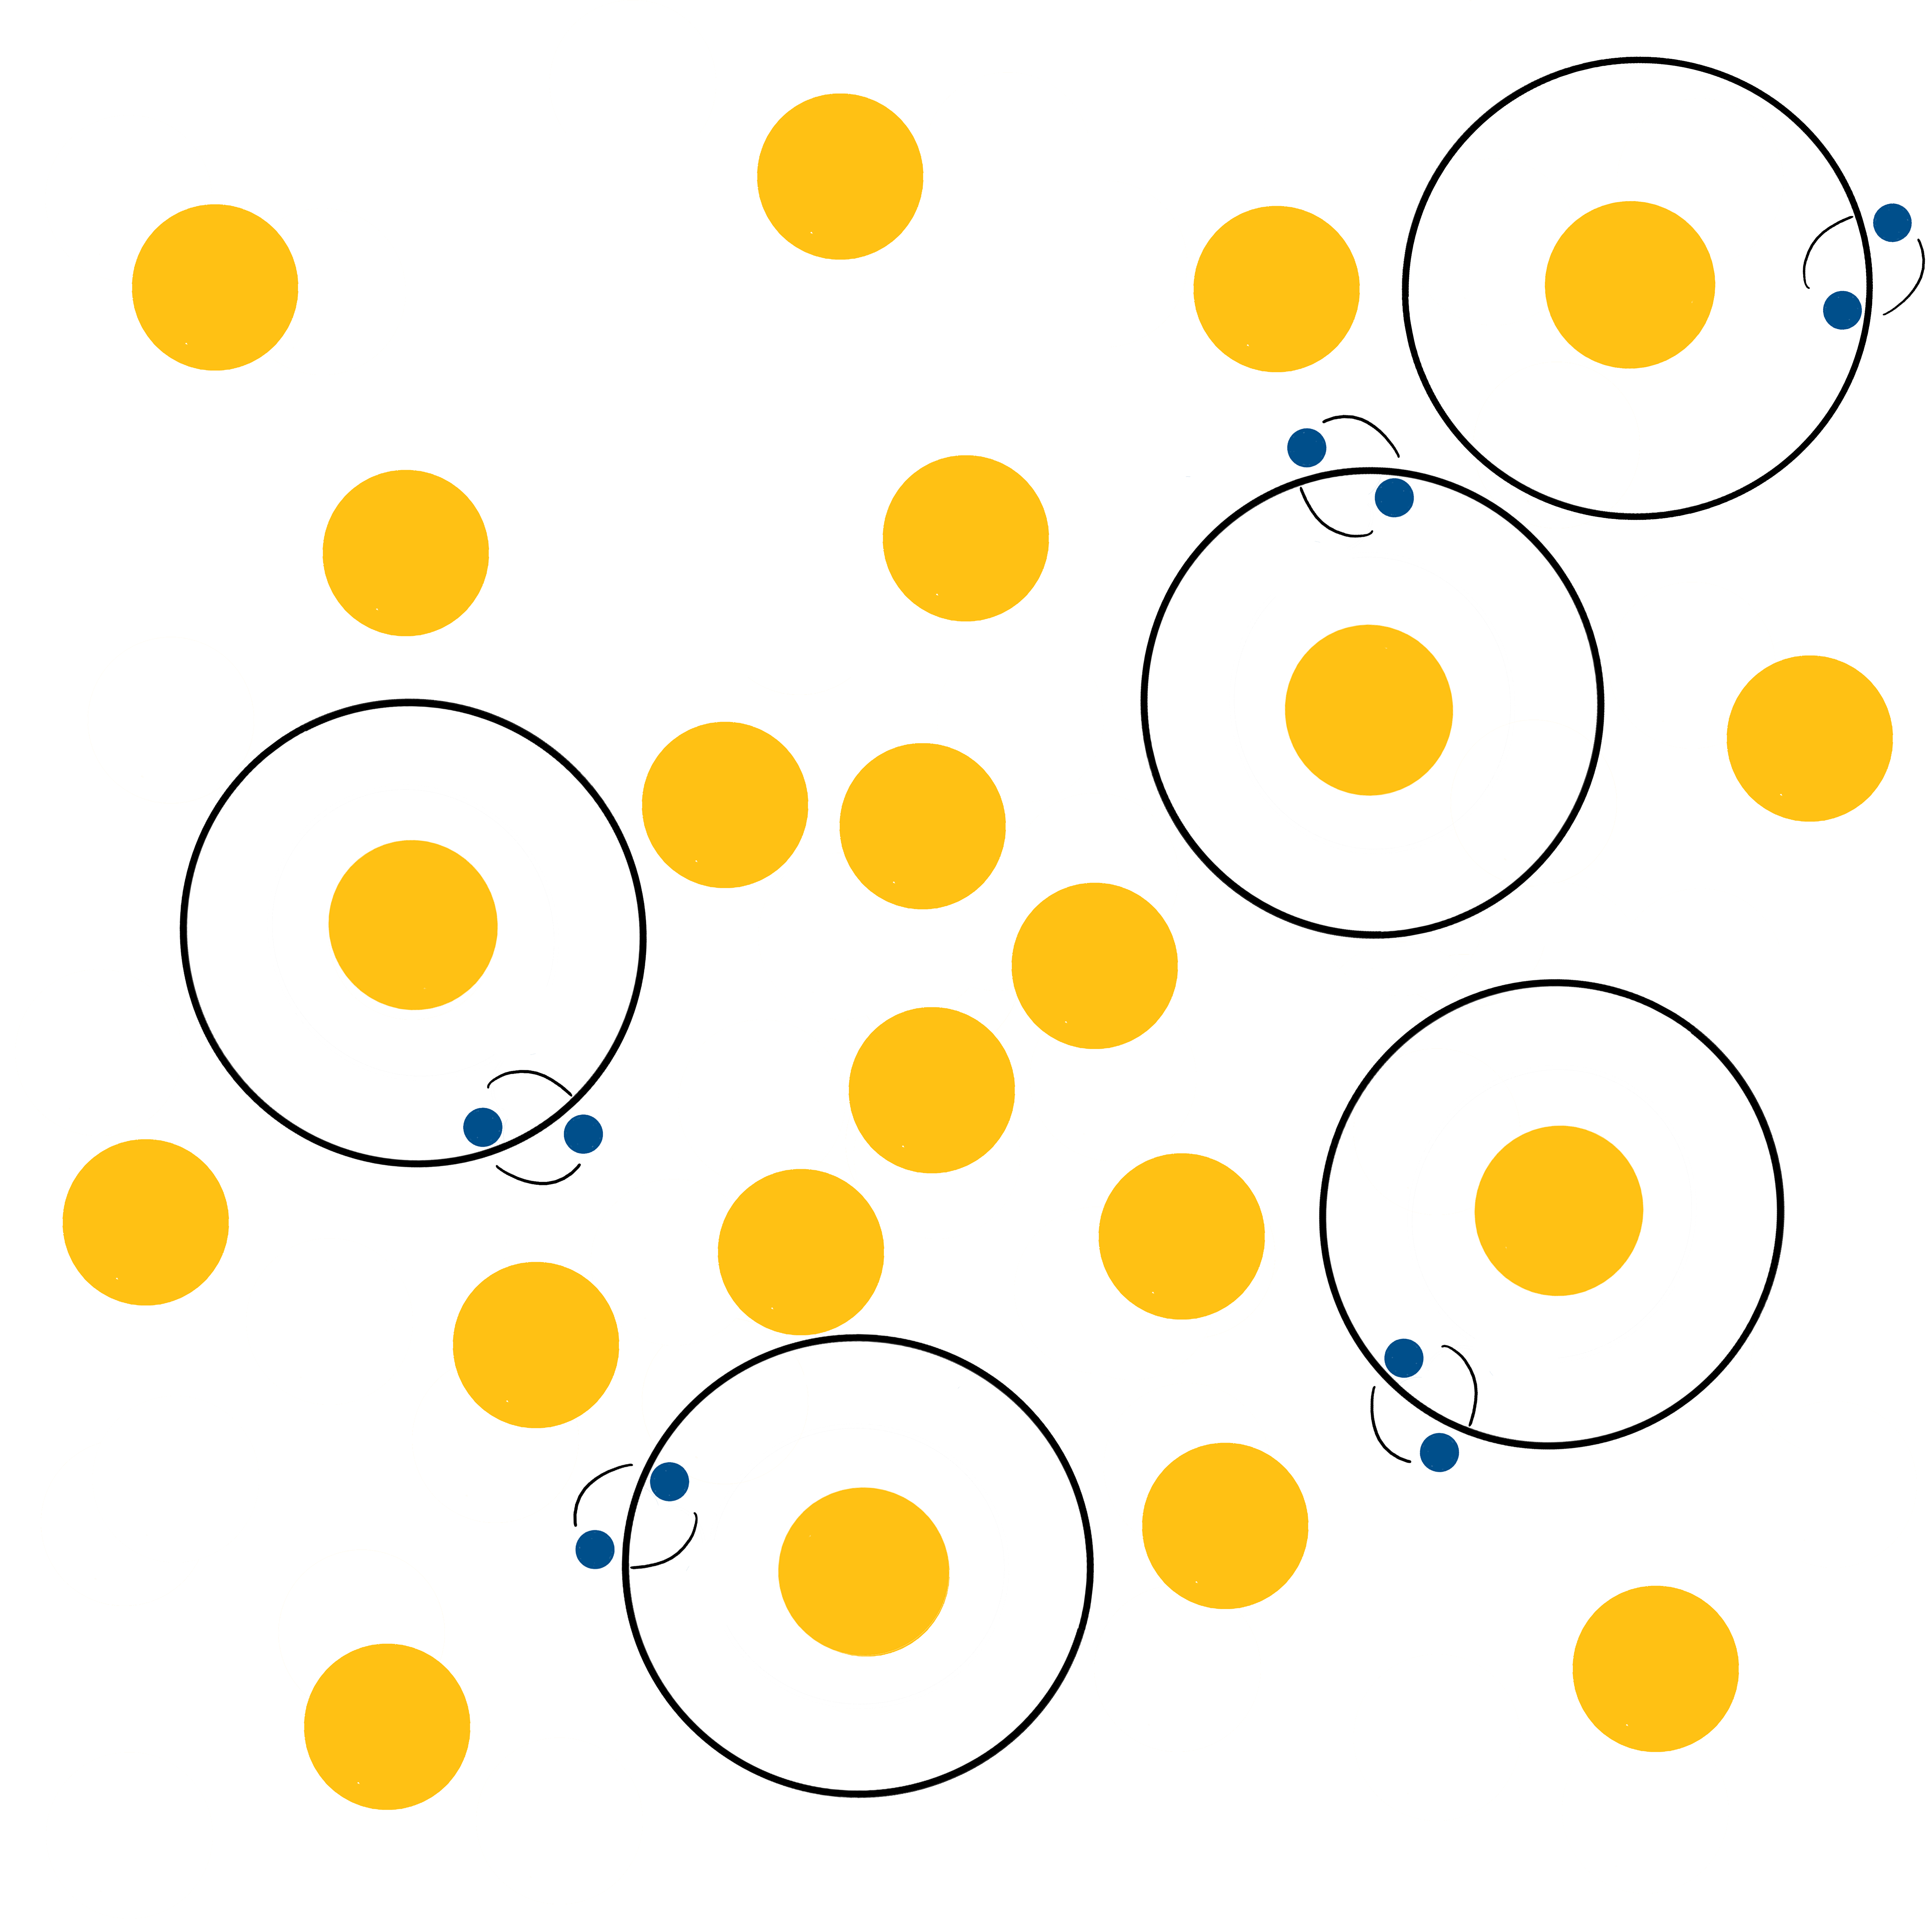
\includegraphics[width=.4\columnwidth]{figures/Model_PM.png}
%% ${\cal FFC}$ 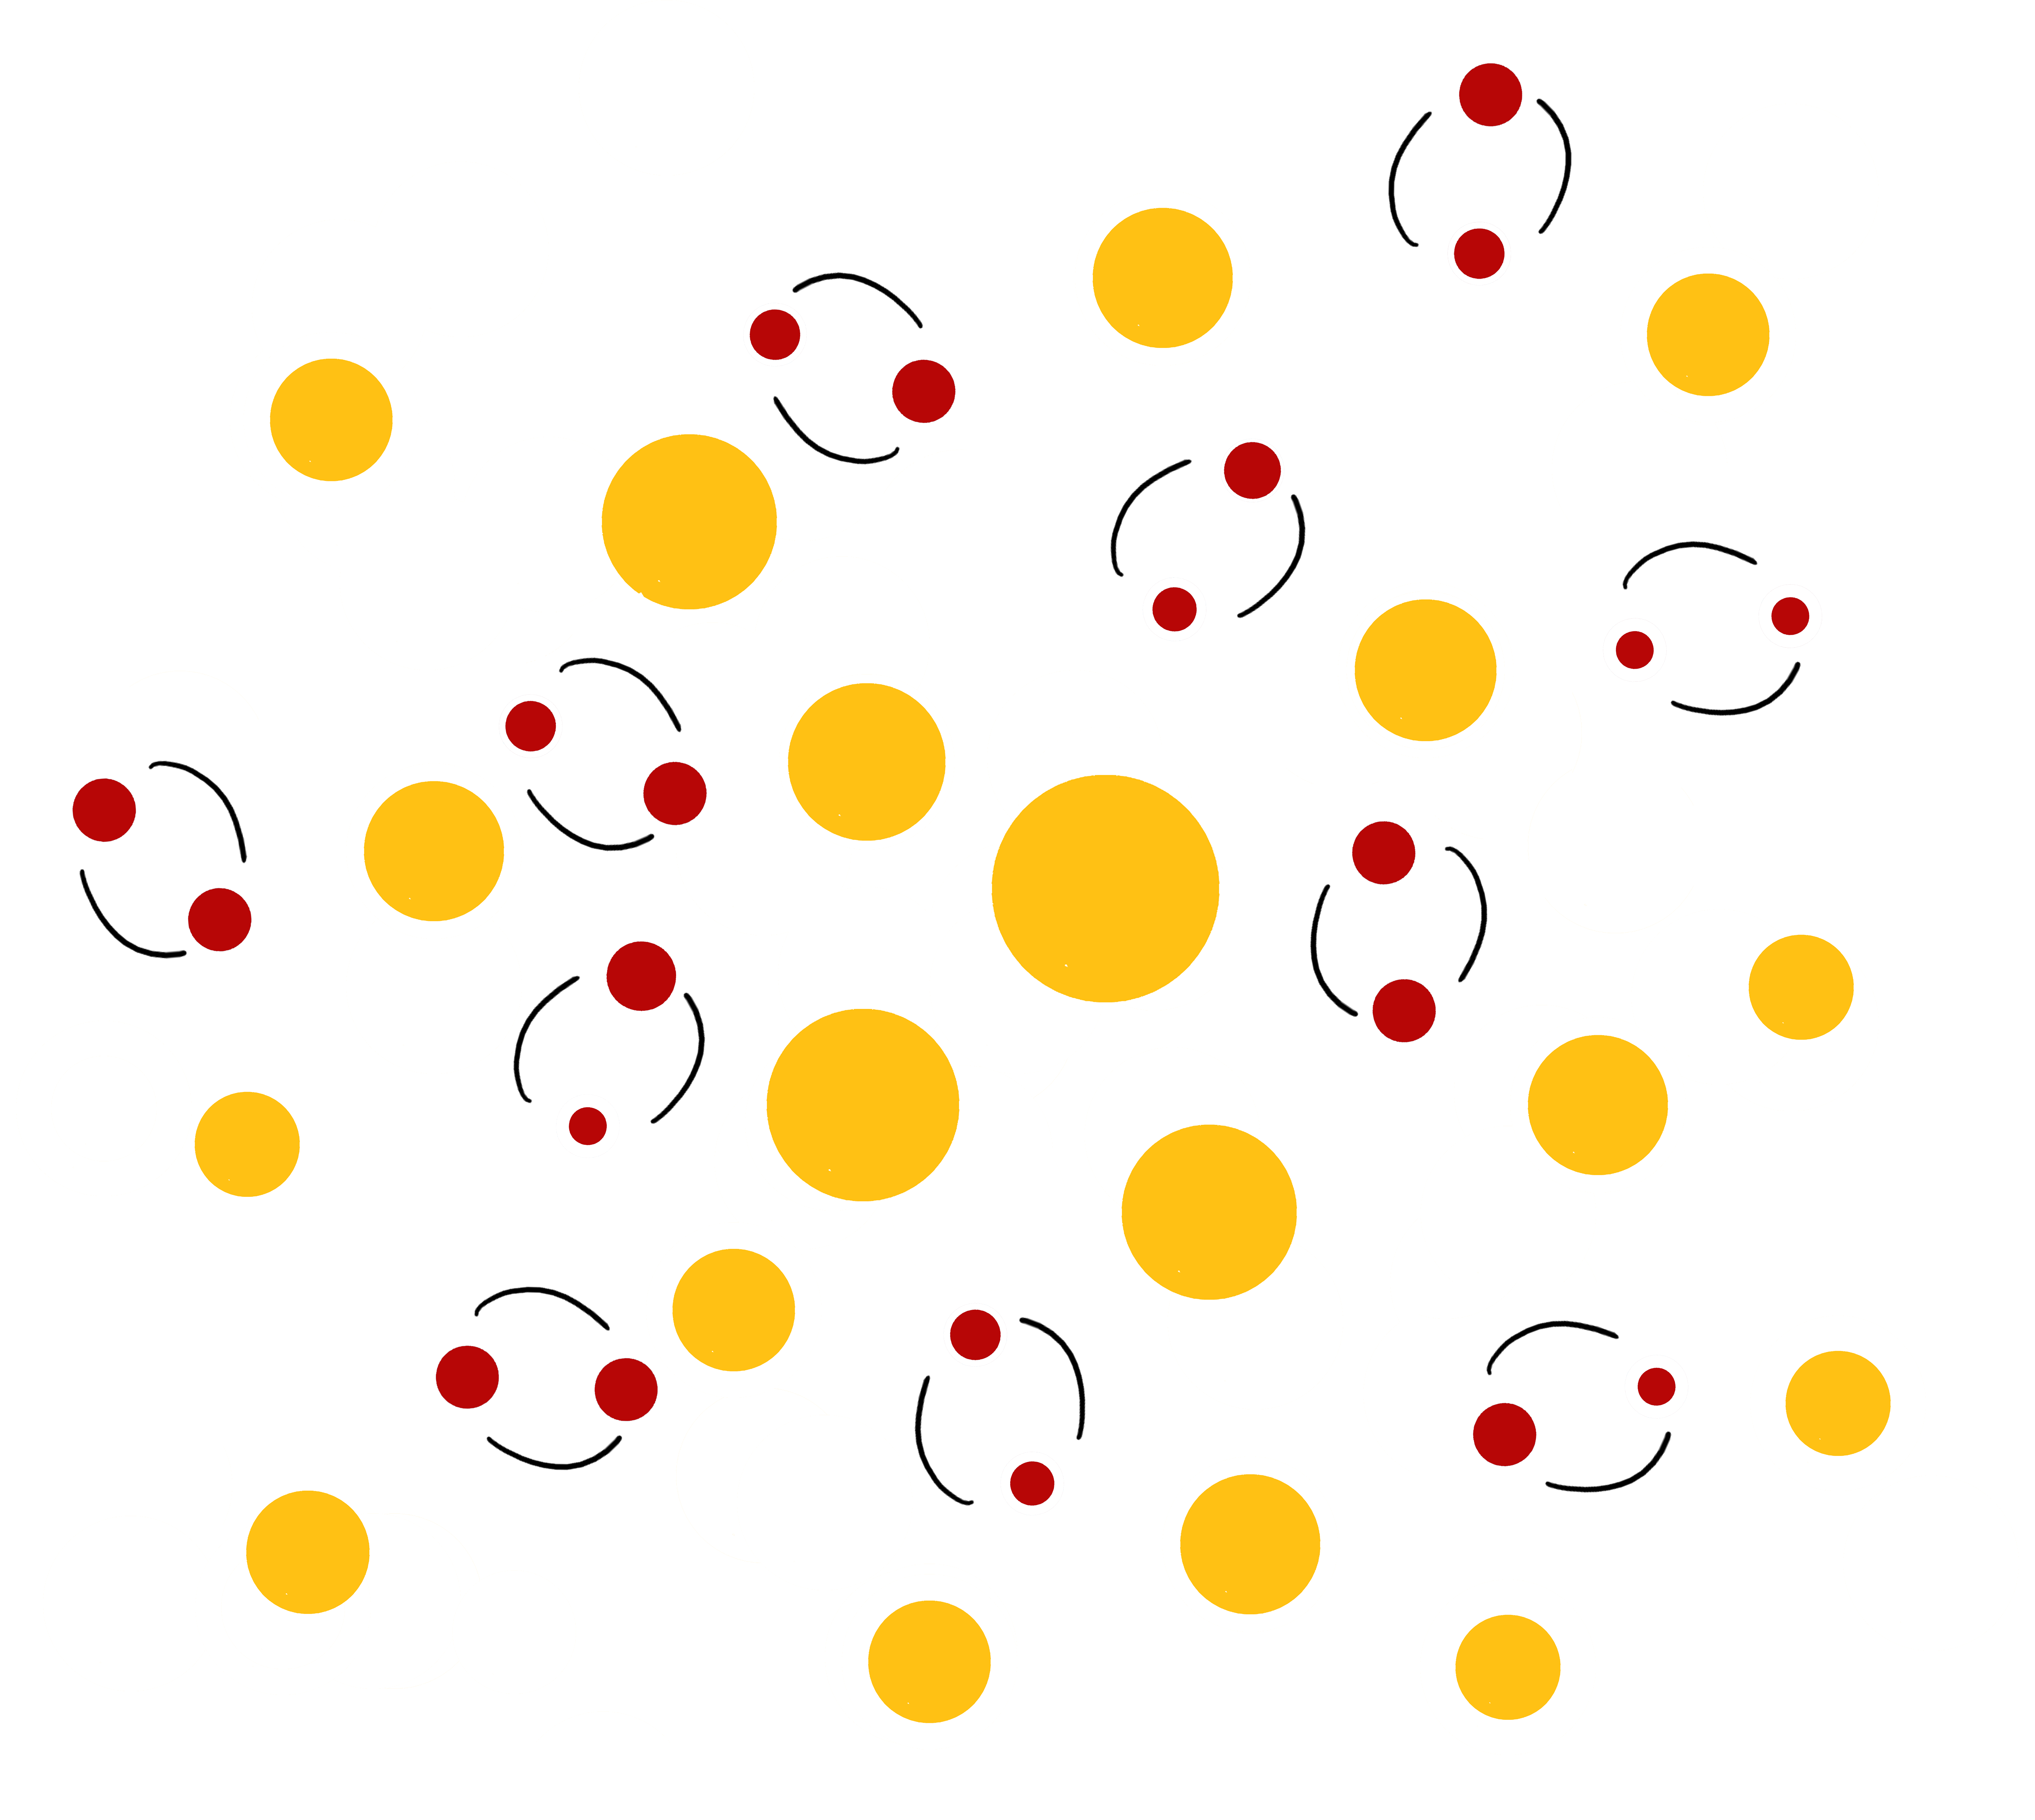
\includegraphics[width=.4\columnwidth]{figures/Model_SF_FFC.png}
%% ${\cal ISF}$ ~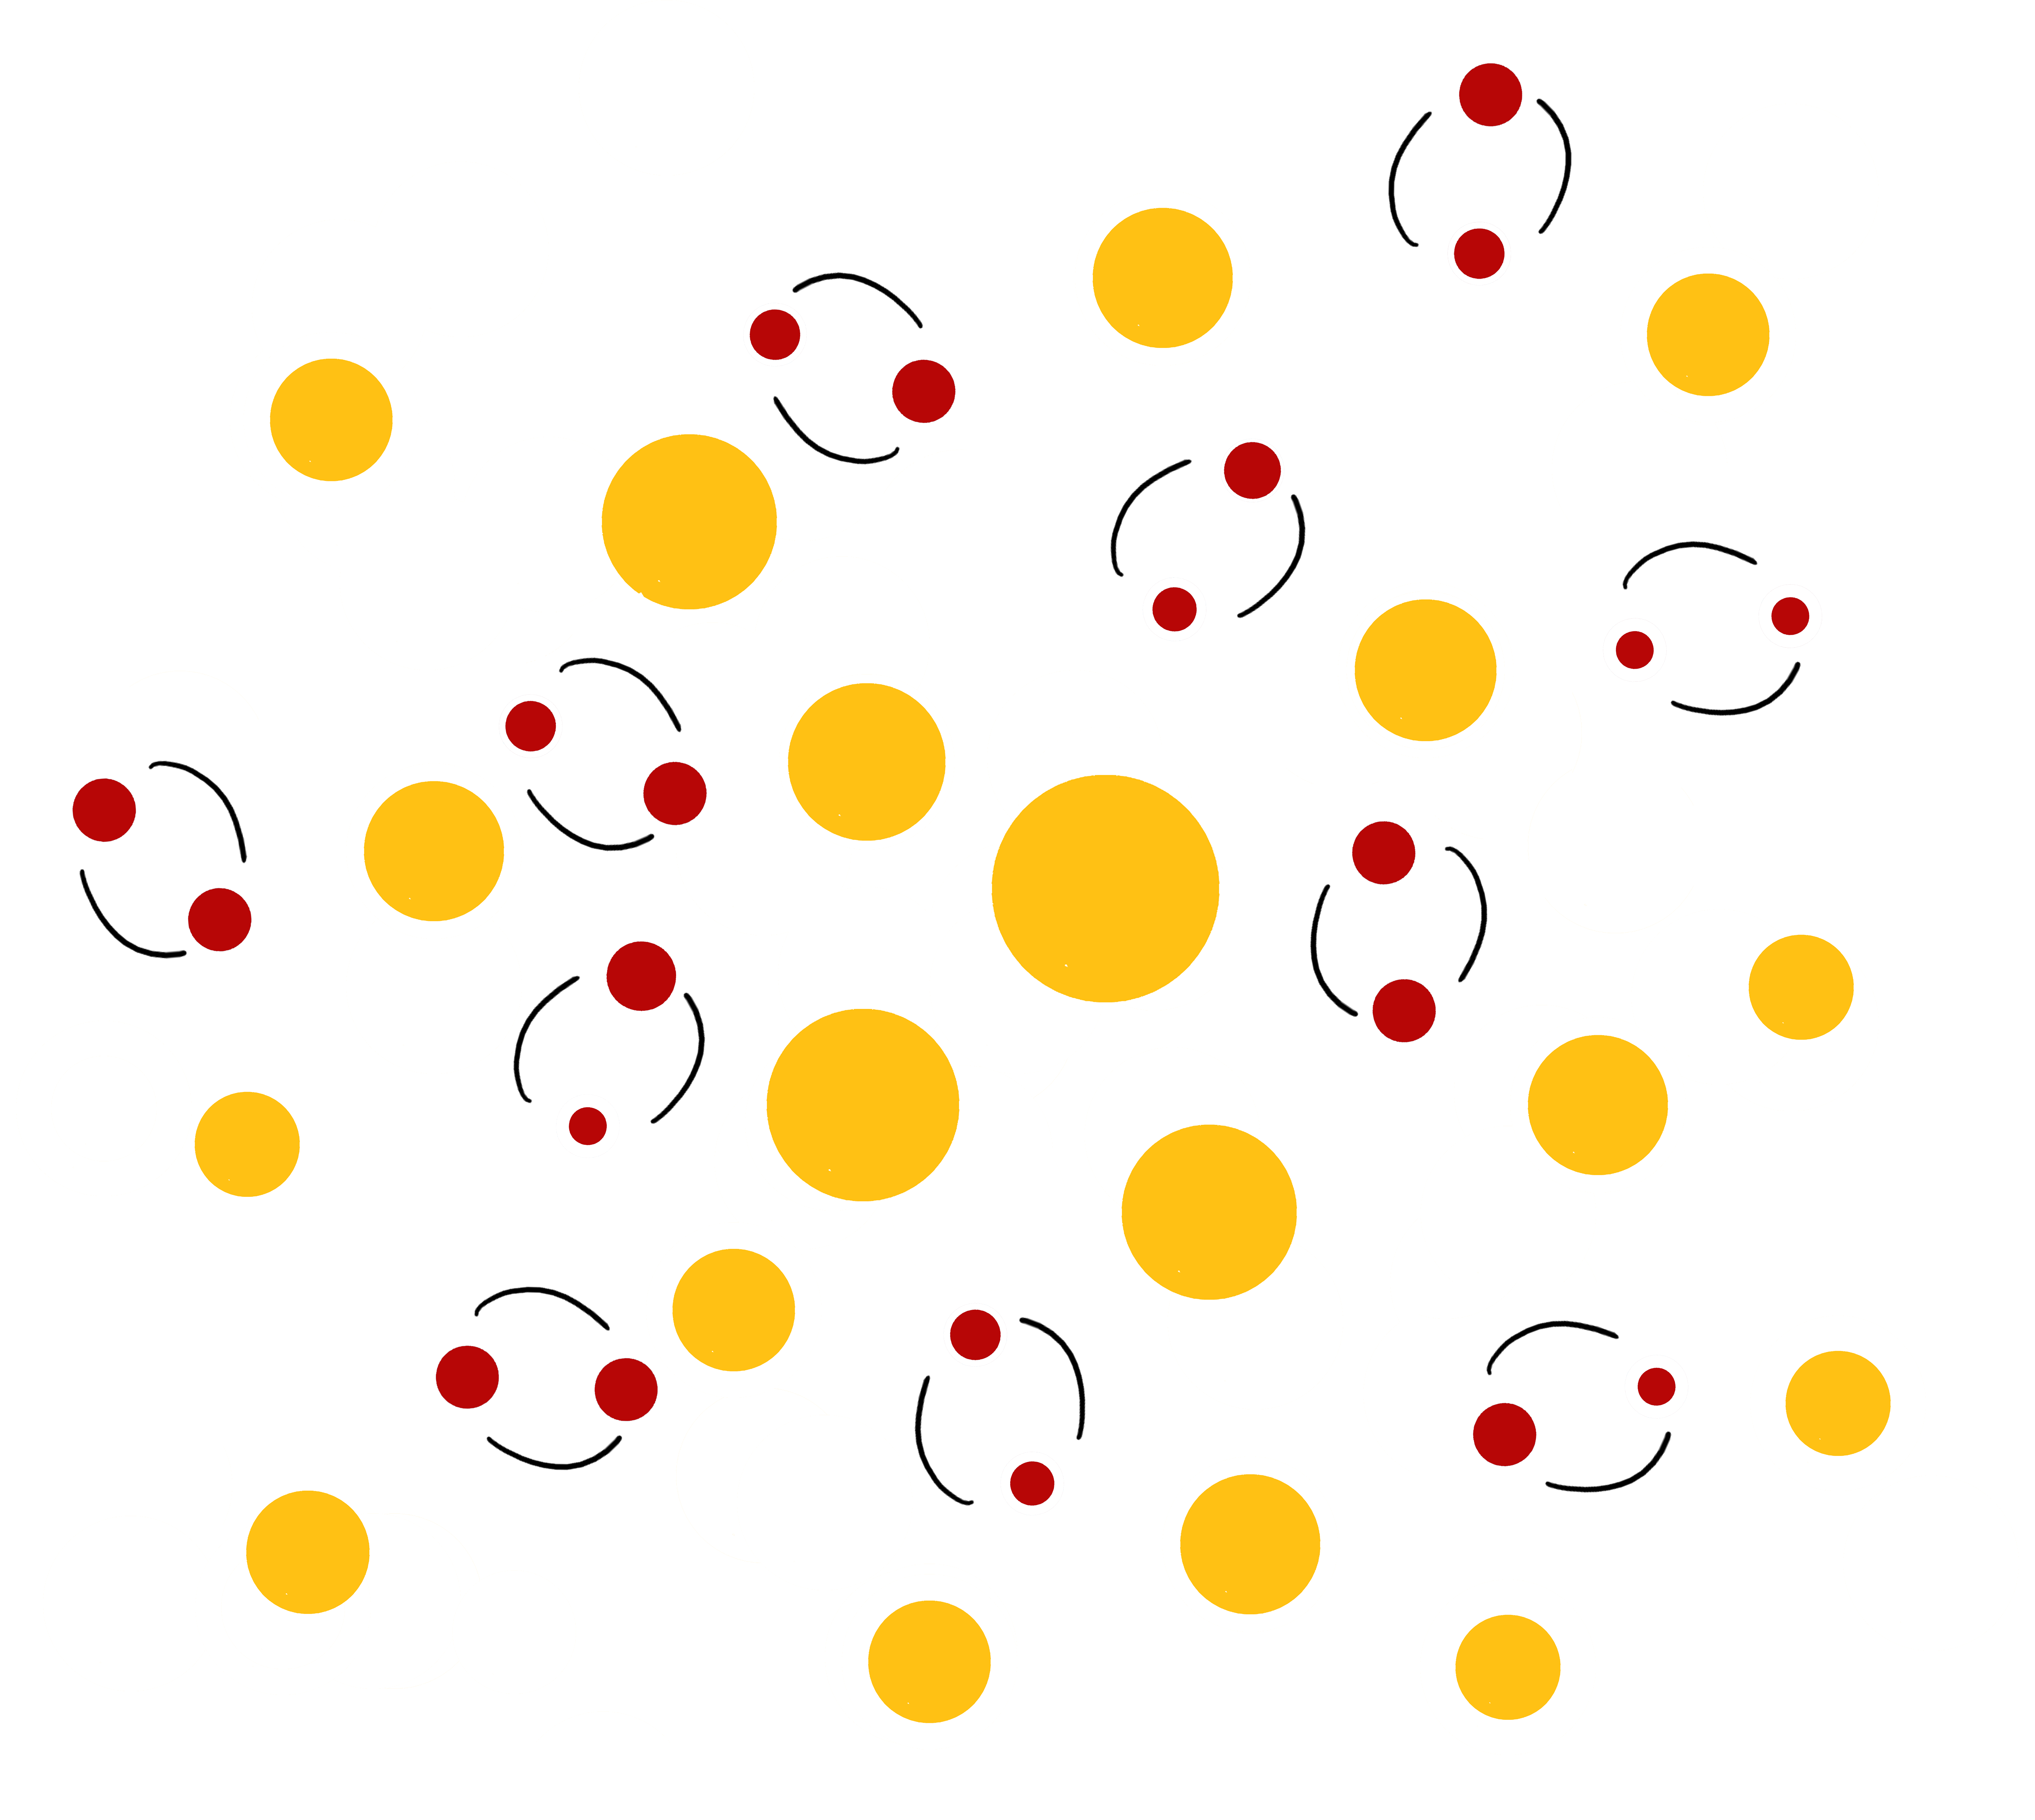
\includegraphics[width=.4\columnwidth]{figures/Model_SF_FFC.png}
%%          \caption{}
%%          \label{Fig:models}
%% \end{figure}

\begin{picture}(100,250)
\put(0,150){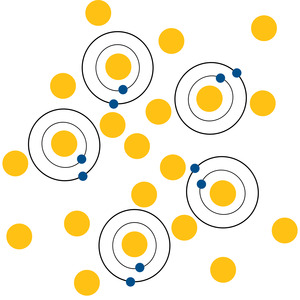
\includegraphics[width=.4\columnwidth]{figures/Model_PP.jpg}}
\put(150,150){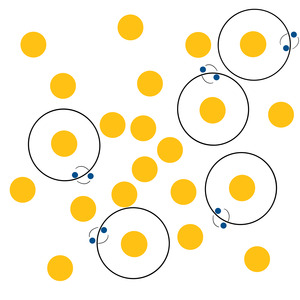
\includegraphics[width=.4\columnwidth,angle=90]{figures/Model_PM.jpg}}
\put(0,0){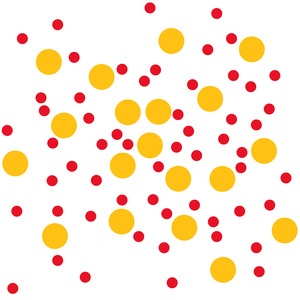
\includegraphics[width=.4\columnwidth]{figures/Model_FFC.jpg}}
\put(150,0){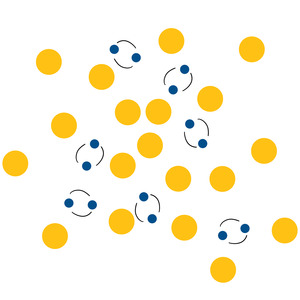
\includegraphics[width=.4\columnwidth,angle=90]{figures/Model_SF.jpg}}
\put(0,150){${\cal SPP}$}
\put(150,150){${\cal SPM}$}
\put(0,0){${\cal FFC}$}
\put(150,0){${\cal ISF}$}
\end{picture}

\subsection{Finding \jumbos}

\jumbos\, are soft in terms of the average local kinetic energy of the
surrounding objects (stars and planets). This complicates the analysis
of the simulation data. We genrally consider hard binary paris or
multiples in direct N-body simulations are finding those soft pairs
requires some extra effort.

\section{Results}

\subsection{Model ${\cal SPP}$}

In scenario ${\cal SPP}$, we follow the dynamical evolution of 1900
single stars, and 300 stars what are hosted by two planets;
potentially forming 600 free-floating JMOs or 300 \jumbos.  According
to \citep{2023arXiv231006016W}, \jumbos\, form naturally upon a
dynamical encounter between the planetary systems and a passing star.
In table\,\ref{Tab:model_numbers} we summarize the results.

\begin{table*}
 \caption{...}
 \label{Tab:model_numbers}
 \centering 
 \begin{tabular}{lrrrrrrrrrrrr}
   \hline\hline
   model & $n_{s}$ & $n_{(s,s)}$ & $n_{(s,p)}$ & $n_{p}$ & $n_{(p,p)}$ \\
        \hline \vspace{-0.75em}\\
${\cal SPP}$\_Pl\_R025 & 2282 &  2 & 214 & 194 & 0  \\
${\cal SPP}$\_Pl\_R050 & 2219 &  0 & 281 &  75 & 0  \\
${\cal SPP}$\_Pl\_R100 & 2206 &  0 & 294 &  15 & 0  \\
${\cal SPP}$\_Fr\_R025 & 2259 & 96 &  10 & 494 & 0  \\
${\cal SPP}$\_Fr\_R050 & 2199 &116 &  39 & 450 & 0  \\ %at t=0.8Myr
${\cal SPP}$\_Fr\_R100 & 2229 & 89 &  64 & 417 & 0  \\ %at t=0.6Myr
 \hline
  \hline \vspace{-0.75em}\\
${\cal SPM}$\_Pl\_R025 & 2473 &  2 &  20 & 289 &  38 \\
${\cal SPM}$\_Pl\_R050 & 2454 &  0 &  37 & 147 & 112 \\
${\cal SPM}$\_Pl\_R100 & 2460 &  0 &  37 &  41 & 156 \\
${\cal SPM}$\_Fr\_R025 & 2337 & 67 &  16 & 300 &  73  \\
${\cal SPM}$\_Fr\_R050 & 2237 &111 &   7 & 365 &  21 \\
${\cal SPM}$\_Fr\_R100 & 2305 & 84 &   6 & 336 &  29  \\
  
  \hline
  \hline \vspace{-0.75em}\\
${\cal ISF}$\_Pl\_R025 & 2498 &   0 &  0 & 363 &  26  \\
${\cal ISF}$\_Pl\_R050 & 2498 &   1 &  0 & 277 &  59  \\
${\cal ISF}$\_Pl\_R100 & 2500 &   0 &  0 & 116 & 130  \\
${\cal ISF}$\_Fr\_R025 & 2270 &  43 & 21 & 279 & ***  \\ %Not finished
${\cal ISF}$\_Fr\_R050 & 2279 &  87 & 13 & 387 &   5 \\
${\cal ISF}$\_Fr\_R100 & 2273 & 101 &  5 & 388 &   6 \\
  \hline
  \hline \vspace{-0.75em}\\
${\cal FFC}$\_Pl\_R025 & 2241 &  98 & 13 & 580 & 0.0  \\
${\cal FFC}$\_Pl\_R050 & 2274 &  97 &  6 & 595 & 0.0  \\
${\cal FFC}$\_Pl\_R100 & 2306 &  80 & 12 & 593 & 0.0  \\
${\cal FFC}$\_Fr\_R025 & 2253 & 103 & 11 & 584 & 0.0  \\
${\cal FFC}$\_Fr\_R050 & 2283 &  99 &  4 & 592 & 0.0  \\
${\cal FFC}$\_Fr\_R100 & 2259 & 106 & 10 & 593 & 0.0  \\
  \hline
 \end{tabular}
\end{table*}


\begin{table*}
  \caption{Simulation results for the models ${\cal SPM} and ${\cal
      FFC}. The other models have an insufficently number of jumbos.}
 \label{Tab:model_parameters}
 \centering 
 \begin{tabular}{llllll}
 \hline\hline
 model & $\langle M \rangle$ & $\langle m \rangle$ & $\langle a \rangle$ & $\langle e \rangle$ & $\langle d \rangle$ \\
 \hline \vspace{-0.75em} \\ 
 ${\cal SPM}$\_Pl\_R025 &$4.099^{+3.445}_{-2.211}$ & $1.204^{+1.587}_{-0.457}$ & $94.541^{+31.133}_{-35.785}$ & $0.381^{+0.217}_{-0.239}$& $79.366^{+33.428}_{-37.153}$  \\
 ${\cal SPM}$\_Pl\_R050 $3.408^{+2.733}_{-1.819}$ & $1.247^{+1.321}_{-0.510}$ & $96.743^{+47.768}_{-36.120}$ & $0.309^{+0.300}_{-0.176}$& $78.471^{+45.944}_{-35.217}$  \\
 ${\cal SPM}$\_Pl\_R100 $3.404^{+3.775}_{-1.647}$ & $1.216^{+1.540}_{-0.500}$ & $118.841^{+38.270}_{-42.641}$ & $0.173^{+0.341}_{-0.112}$& $91.384^{+49.231}_{-34.896}$  \\
 ${\cal SPM}$\_Fr\_R025 &$4.546^{+3.993}_{-2.676}$ & $1.311^{+1.473}_{-0.670}$ & $138.080^{+57.671}_{-64.512}$ & $0.385^{+0.209}_{-0.229}$& $111.158^{+88.174}_{-60.725}$  \\
 ${\cal SPM}$\_Fr\_R050 &$8.772^{+1.495}_{-5.261}$ & $2.229^{+2.105}_{-1.319}$ & $63.796^{+61.614}_{-6.539}$ & $0.564^{+0.168}_{-0.288}$& $58.856^{+24.145}_{-20.651}$  \\
 ${\cal SPM}$\_Fr\_R100 &$4.291^{+4.876}_{-2.006}$ & $2.021^{+1.131}_{-1.121}$ & $64.022^{+121.340}_{-18.722}$ & $0.418^{+0.103}_{-0.228}$& $66.118^{+49.924}_{-29.847}$  \\
 \hline \vspace{-0.75em} \\ 
 ${\cal ISF}$\_Pr\_R025 &$7.038^{+4.386}_{-4.392}$ & $2.342^{+2.062}_{-1.197}$ & $129.908^{+202.916}_{-56.779}$ & $0.447^{+0.181}_{-0.081}$& $109.341^{+131.269}_{-53.461}$  \\
 ${\cal ISF}$\_Pl\_R050 &$5.641^{+4.416}_{-2.957}$ & $2.017^{+1.577}_{-0.820}$ & $272.202^{+193.815}_{-146.941}$ & $0.603^{+0.146}_{-0.200}$& $222.387^{+184.742}_{-112.468}$  \\
 ${\cal ISF}$\_Pl\_R100 &$4.346^{+2.984}_{-2.310}$ & $1.490^{+1.685}_{-0.503}$ & $434.625^{+216.002}_{-254.635}$ & $0.657^{+0.130}_{-0.221}$& $327.553^{+270.306}_{-184.532}$  \\
 ${\cal ISF}$\_Fr\_R025 &$5.612^{+3.713}_{-3.042}$ & $1.770^{+1.381}_{-0.807}$ & $39.134^{+28.750}_{-13.735}$ & $0.619^{+0.176}_{-0.220}$& $37.378^{+27.504}_{-19.258}$  \\
 ${\cal ISF}$\_Fr\_R050 &$2.793^{+4.333}_{-1.069}$ & $0.932^{+1.792}_{-0.098}$ & $48.820^{+0.281}_{-22.500}$ & $0.782^{+0.056}_{-0.030}$& $56.751^{+22.579}_{-30.176}$  \\
 ${\cal ISF}$\_Fr\_R100 &$4.626^{+3.611}_{-1.883}$ & $1.853^{+1.798}_{-0.778}$ & $47.969^{+20.671}_{-24.135}$ & $0.617^{+0.200}_{-0.162}$& $38.419^{+31.666}_{-20.512}$  \\
 \hline \vspace{-0.75em}  \\
 \end{tabular}
\end{table*}

The ${\cal SPP}$ model fails to reproduce the observed population of
\jumbos\, by a factor of 50 to 400.  The proportion of \jumbos\,
relative to free-floating JMO's is lower than observed values by a
factor of 100. Moreover, their orbits are considerably tighter.
Changing the initial distribution in semi-major axis of the inner
orbit from a uniform distribution to a logarithmic distribution
reduces the formation rate of \jumbos\, even further.

To further explore the failure of model ${\cal SPP}$, we perform an
additional series of simulations with pre-determined inner and outer
orbital separations $a_1$ and $a_2$ using the Plummer distribution
with virial radii of 0.25\,pc, 0.50\,pc and 1.0\,pc for the stars.
According to \citep{2023arXiv231006016W}, the eventual orbital
separation of the \jumbo\, would be consistent with the difference in
orbital separation between the two planets when orbiting the star. For
this reason we perform an additional series of runs with a mutual
separation $a_2-a_1 = 200$\,au, expecting those to lead to consistent
results in comparison with the observations.  The results of these
simulations are presented in figure\,\ref{Fig:fjumbos_from_PP}.

For these models the \jumbo-formation efficiency peaks for an orbital
separation $a_1 \apgt 1000$\,au, but steeply drops for smaller values
of $a_1$. As proposd by \citep{2023arXiv231006016W}, we adopt a
difference in the initial orbital distance of about $a_2-a_1 =
100$\,au or 200\,au (see figure\,\ref{Fig:fjumbos_from_PP}), which
would lead to \jumbo\, orbits in the same range.  We performed a total
of 45 calculations with various ranges of $a_1$ and $a_2$, of which 39
produced a total of 910 \jumbos. The initial mean value of $a_1-a_2 =
167\pm38$\,au, leading to a final orbital separation of the jumbos of
$a_j \sim 262\pm45$\,au.  The claim made by
\citep{2023arXiv231006016W}, that the separation distance $a_2-a_1$
leads to \jumbos\, with a similar orbital distance seems reasonable.

The rate, derived by \citep{2023arXiv231006016W}, however, appears to
be orders of magnitude smaller than they expected.  They calculate the
rate by means of 4-body scattering experiments, in which a star with
two equal-mass planets with semi-major axes $a_1$ for the inner and
$a_2$ for the other planet, encounters a single star. Their largest
cross section of roughly $a_1^2$ is obtained if the encounter velocity
$0.8v_\star/v_1$. For an encounter at the cluster's velocity
dispersion, the inner planet would then have a orbital separation of
about 900\,au around a 1\,\MSun\, star.

\begin{figure}
    \centering
        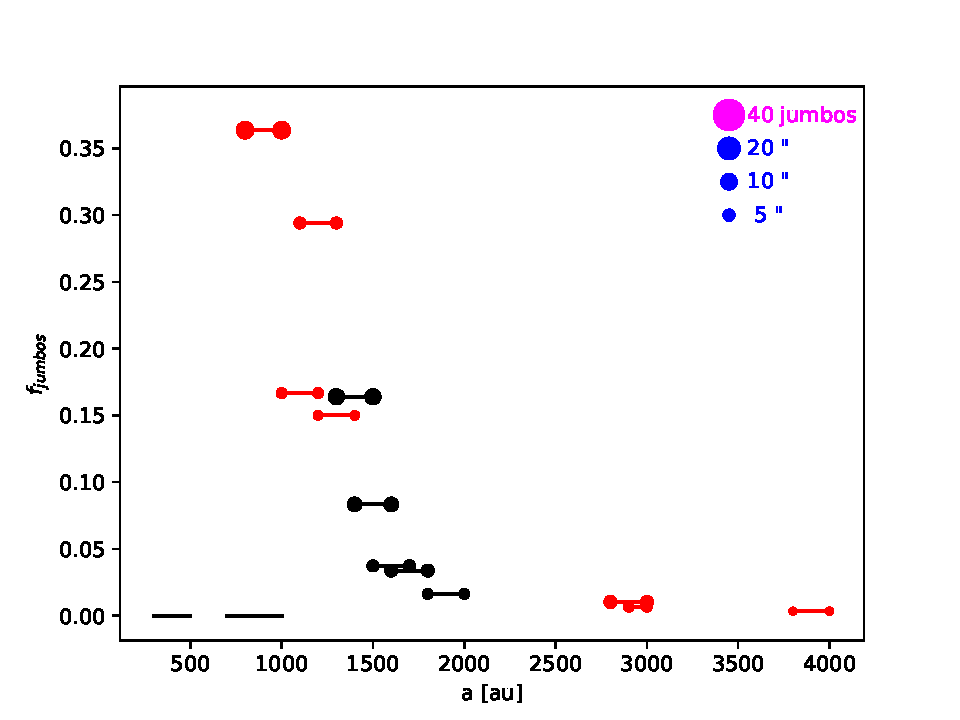
\includegraphics[width=.91\columnwidth]{figures/fig_fjumbos_from_psystems.pdf}
        \caption{The number of jumbo's produced in model ${\cal SPP}$,
          as fraction of the number of free floating planets for
          various simulations starting with a Plummer sphere with a
          virial radius of 0.5\,pc.  The bullet points along each line
          correspond with the adopted orbital separation of the two
          planets ($a_1$ and $a_2$).  The red symbols indicate an
          average orbital separations for the jumbos between 25\,au
          and 380\,au.  The black symbols are outside this regime.
          The symbol sizes give the number of jumbos (see top right
          for scaling) in the particular simulation.  }
         \label{Fig:fjumbos_from_PP}
\end{figure}

\subsection{Model ${\cal SPM}$}

In the ${\cal SPM}$ models we initialize planet pairs (or planet with
moons) in orbit around a star. The planet-moon system orbit was
selected to mimic the observed distribution of \jumbos\, and therefore
are generally rather wide ($a \sim 200$\,au). But we adopted
relatively circular orbits ($e<0.02$) for the planet-moon pair.  To
warrant stability of the star-planet-moon system, we chose an orbital
separation such that the planet-moon pair stays witin 1/3th of it's
Hill radius in orbit around the star. As a consequence, these systems
are generally rather wide, and therefore fragile for being stripped in
encounters with other stars. At the same time, the planet-moon pairs
tend to be soft, much in the same way as the observed \jumbos\, are
soft. This is reflected in the rate and orbital parameters of the
\jumbos\, resulting from model ${\cal SPM}$.

In model ${\cal SPM}$ we find an abundance of \jumbos\, with about 500
per cluster when we start with a Plummer distribution, and about 100
for the fractal models (starting with 600 pairs). The lower frequency
for the fractal models reflects the more dynamic environment in which
\jumbos\, are easily ionized. This trend is also noticeable in the
number of stellar binaries and free floating planets, but also in the
\jumbo\, orbital parameters. \jumbos\, originating from the Plummer
models tend to be rather circular and somewhat wider than those
surviving in the fractal model.  These trends are indepenedend of the
cluster density (or virial radius). We do expect some difference in
the \jumbo\, population as a fuction of the initial cluster density,
but the distribution \jumbo\, parameters in the simulations are wide
and they probaby do not form the right population to make such a
distinction.

\subsection{Model ${\cal FFC}$}


\subsection{Model ${\cal ISF}$}

\begin{figure}
    \centering
        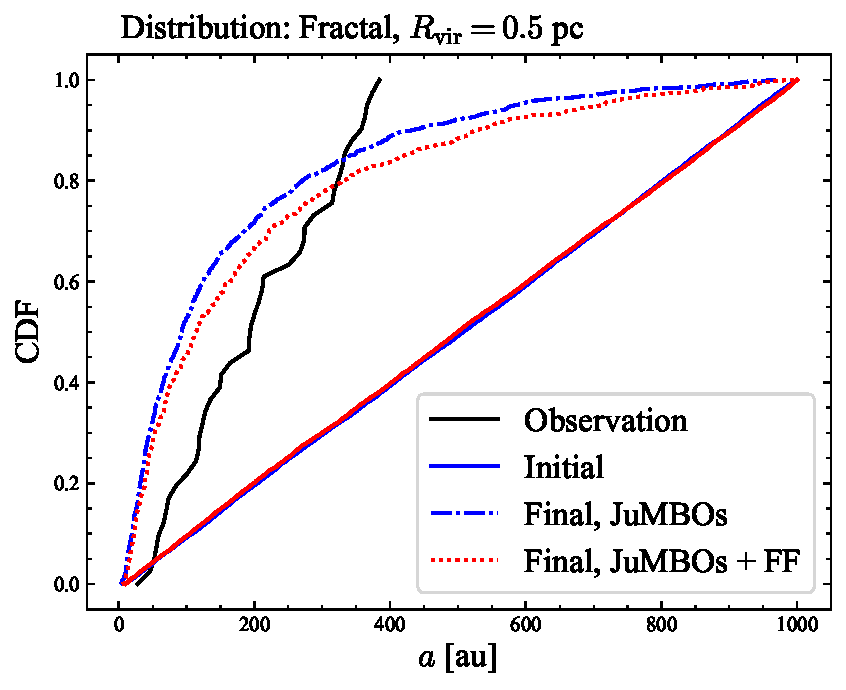
\includegraphics[width=.91\columnwidth]{figures/sem_axis_Fractal_FF.pdf}
        \caption{}
         \label{Fig:Fr_semimajor_axis}
\end{figure}

\begin{figure}
    \centering
        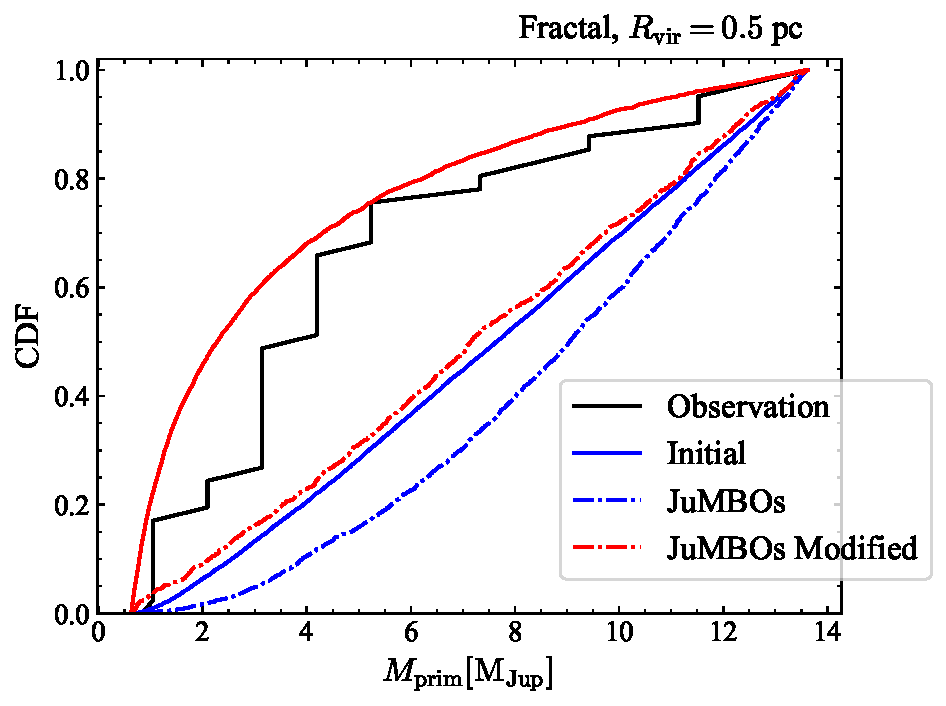
\includegraphics[width=.91\columnwidth]{figures/mprim_vs_obs_Fractal0.5Mod.pdf}
        \caption{}
         \label{Fig:Fr_primar_mass}
\end{figure}

\begin{figure}
    \centering
        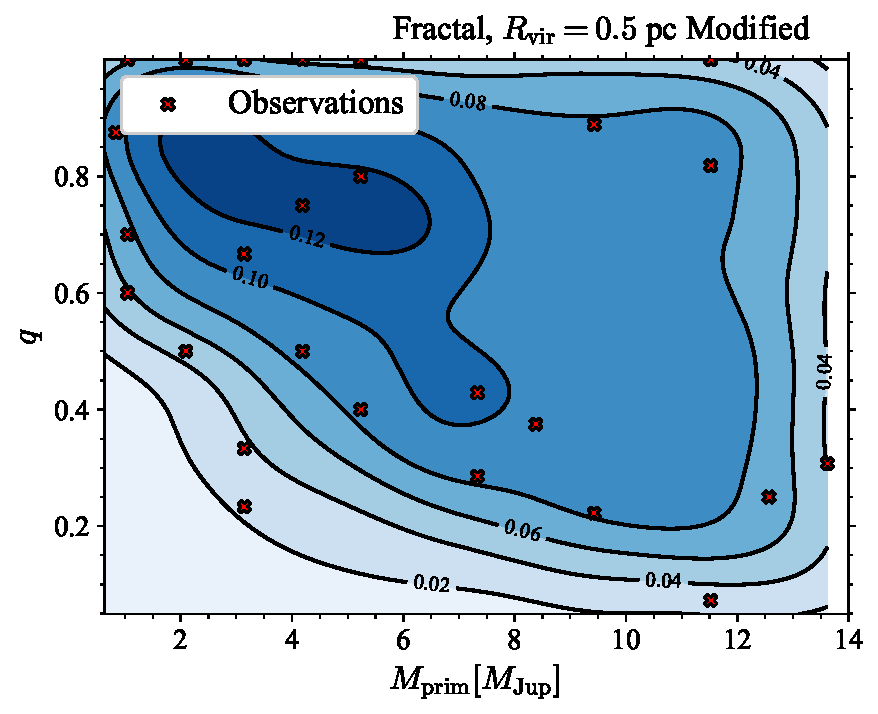
\includegraphics[width=.91\columnwidth]{figures/mass_distr_Fractal_rvir0.5_mod_params.pdf}
        \caption{}
         \label{Fig:Fr_mass_ratio_distribution}
\end{figure}

\begin{figure}
    \centering
        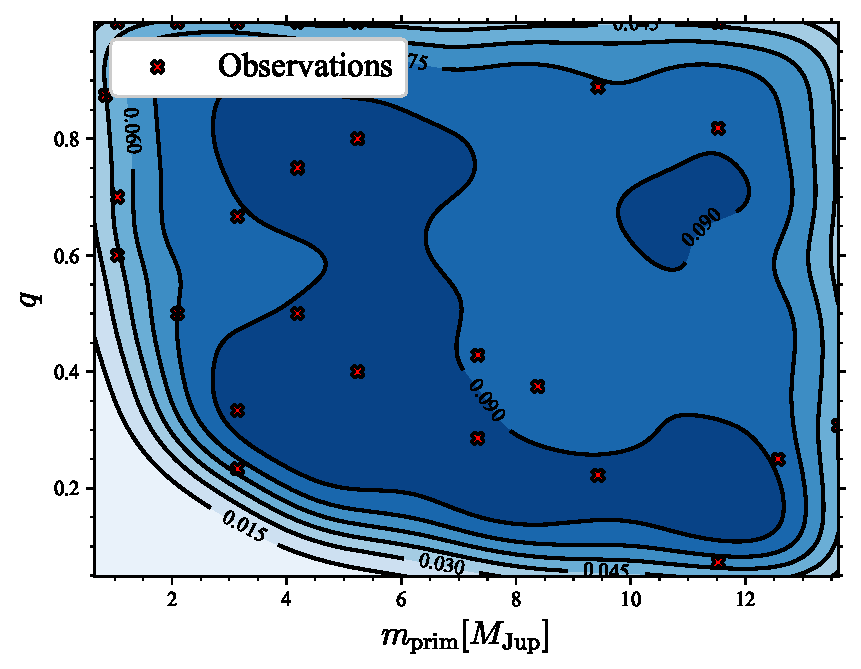
\includegraphics[width=.91\columnwidth]{figures/mass_distr_Plummer_rvir0.5.pdf}
        \caption{}
         \label{Fig:Plummer_massfunction}
\end{figure}
\begin{figure}
    \centering
        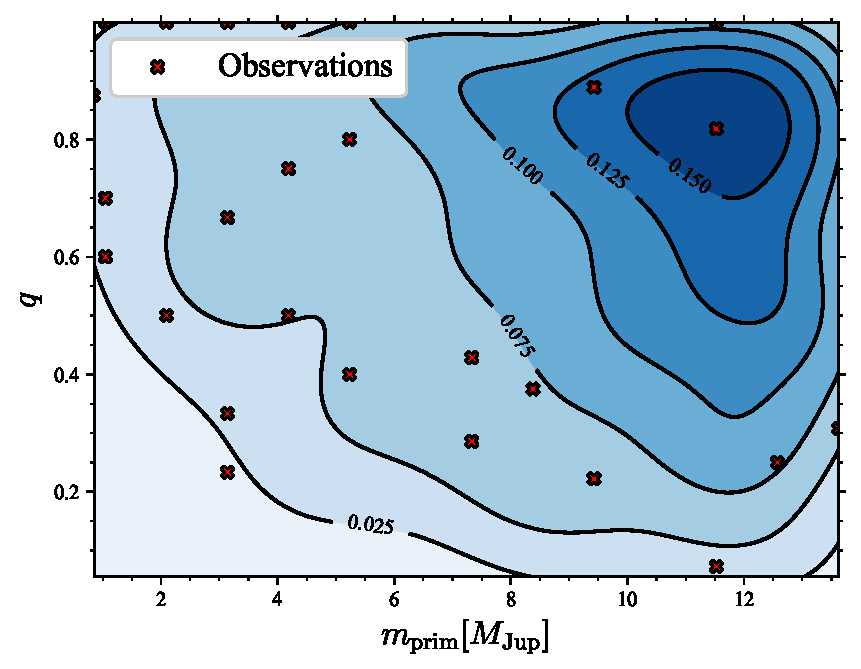
\includegraphics[width=.91\columnwidth]{figures/mass_distr_Fractal_rvir0.5.pdf}
        \caption{}
         \label{Fig:fractal_massfunction}
\end{figure}



\subsection{stellar and planetary collisions}

No collisions occur between stars or planets in a Plummer models,
where in the fractal models collisions these events become rather
common.

in the ${\cal SPM}$ models $12.9\pm8.0$ stars experienced a collision
with another star. No planets collided with other planets, or with a
star.


\section{Discussion}


\citep{2023arXiv231015603C} argued that \jumbos\, potentially originate
from tilted circum-binary planets. Formed as a --sort-of-- planet-moon
system in a wide orbit around a star, that is strippied from the host
star by the cluster potential or a relatively wide encounter with
another star. 


Single free floating planetary objects were discovered in abundance
(between 70 and 170 candidates) before in the Upper Scorpius
association \citep{2022NatAs...6...89M}, but these were considered to
be single free floaters.  With an age of about 11\,Myr \citep{++},
Upper Scorpio is expected to be rich in single jupiter mass free
floating planets, but binaries will be rare as these have been broken.

The orbital parameters of the \jumbos\, hardly seem to depend on the
cluster density (or virial radius). We do expect some difference in
the \jumbo\, population as a fuction of the initial cluster density,
but the distribution \jumbo\, parameters are wide and they probaby do
not form the right population to make such a distinction.

\subsection{The failure of model ${\cal SPP}$}

Note that an inner orbital separation of $a_1=800$\,au for a
10\,\MJup\, planet leads to a Hill radius of about 150\,au. An orbit
with $a_2=1000$\,au, is probably only marginally stable.  Still,
even in those runs the total number of \jumbos\, remains small
compared to the number of free floaters.

In \citep{2023arXiv231006016W}, the highest cross section is achieved
for the orbital velocity of the inner-most planet as fraction of the
typical encounter velocity $v1/v_{\rm disp} \sim 0.8$. With a cluster
velocity dispersion of $\sim 0.8$\,km/s, the orbital velocity roughly
1\,km/s. Around an 1\,\MSun\, star such a velocity is obtained,
assuming a Kepler orbit, at an orbital separation of 800\,au. It turns
out, that the results of the cross section calculations performed by
\citep{2023arXiv231006016W} are consistent with our direct N-body
simulation, but that the adopted initial orbital separation is too
wide in comparison with a realistically population of inner planetary
orbits for jupiter-mass planets.  Observational selection effect in
finding $\apgt 800$\,au jupiter-mass planets are quite severe, but we
consider it unrealistic to have 600 out of 2500 stars to be orbited by
such wide planetary systems. In particular, when one considers the
small sizes of the observed disks in the Trapezium cluster, which
today are all smaller than 400\,au \citep{2005A&A...441..195V}.

\subsection{\jumbos\, as former planet-moon pairs, model {\cal SPM}}


\subsection{\jumbos\, as former multi-planet systems, model {\cal SPP}}

According to \citep{2023arXiv231015603C}, jumbos form naturally upon a
dynamical encounter between two stars one of which with orbited by a
binary planet or planet-moon system.

Both calculations \citep{2023arXiv231006016W} and
\citep{2023arXiv231015603C} adopt scattering experiments to determine
the formation rate of jumbos from their adopted initial conditions.

\subsection{\jumbos\, formed for capture of free-floating planets, model {\cal FFC}}

\subsection{\jumbos\, as primoridal low-mass object pairs, model {\cal SPP}}


Recently 
70 to 170 candidates) before in the 10\,Myr old association
Upper Scorpius \citep{2022NatAs...6...89M}, but these were considered
to be single. 

\subsubsection{Further constraining the initial conditions}
Using the results of the general models, we alter our initial
conditions with the aim of mimicking observations. Doing so allows us
to disentangle aspects of the cluster history, allowing for
predictions on the properties of \jumbo\, formation. These runs
correspond to the middle segment of table \ref{Tab:SF_FF_Params}.
    
For all models, we constrain $N_{\mathrm{JuMBO}} + N_{\mathrm{FF}}$ to
values reflecting the total planetary-mass population observed in
\citet{2023arXiv231001231P}, keeping in mind the survival rate of
JuMBO systems based on previous results to decide on the initial value
of $N_{\mathrm{JuMBO}}$. The range of mass ratio and mass value
remains unchanged. However, now the mass ratio follows a thermal
distribution to reflect the abundance of $q=1$ observations, whilst
the mass of the objects follows a power-law distribution with $\alpha
= -1.2$. The semi-major axis is uniformly distributed between the
restricted range $a\in[25,100]$ au. Here, the lower bound reflects the
restrictions of observational resolution in the original study
\citep{2023arXiv231001231P}.
    
Models `F050C' and `F0FFOC' look at scenarios where the initial JuMBO
population has an eccentricity ranging between $e\in[0,0.2]$ sampled
from a uniform distribution. For all other models, the eccentricity
remains thermalised and ranges between $e\in[0,0.9]$.
 
\begin{table}
  \caption{Initial conditions of the various configurations. The
    nomenclature is as follows: The first letter identifies the
    cluster distribution. The number denotes the initial virial
    radius, `FF' denotes the presence of Jupiter-mass free floaters,
    `x' whether the system contains an abundance (excessive/extra)
    amount of these free floaters, `O' denotes systems whose JuMBOs
    have their initial parameters constrained by the observational
    data and finally `C', systems whose initialised \jumbos\, are on
    circular orbits. Column 1: The model used. Column 2: The number of
    simulations for the given configuration. Column 3: The initial
    virial radius of the system. Column 4: The number of initialised
    JuMBOs. Column 5: The number of initialised free floaters.}
        \label{Tab:SF_FF_Params}
        \centering 
        \begin{tabular}{c c c c c c}
        \hline\hline
        Model & $N_{\mathrm{runs}}$ & $R_{\mathrm{vir}}$ [pc] & $N_{\mathrm{JuMBO}}$ & $N_{\mathrm{FF}}$\\
        \hline \vspace{-0.75em}\\ 
           F05     & $20$ & $0.5$ & $500$ & $0$ \\
           F05FF   & $20$ & $0.5$ & $500$ & $500$ \\
           F1      & $20$ & $1.0$ & $500$ & $0$ \\
           P05     & $20$ & $0.5$ & $500$ & $0$ \\
           P05FF   & $20$ & $0.5$ & $500$ & $500$ \\
           P1      & $20$ & $1.0$ & $500$ & $0$ \\
           \hline
           \hline \vspace{-0.75em}\\
           F05O   & $10$ & $0.5$ & $275$ & $0$ \\
           F05FFO & $10$ & $0.5$ & $170$ & $400$ & \\
           F05OC   & $10$ & $0.5$ & $275$ & $0$ \\
           F05FFOC & $10$ & $0.5$ & $170$ & $400$ & \\
           P05FFO   & $10$ & $0.5$ & $60$  & $500$ \\
           \hline
           \hline \vspace{-0.75em}\\
           F05FFxJ & $5$ & $0.5$ & $500$ & $10^{4}$ \\
           F05FFx  & $5$ & $0.5$ & $0$   & $10^{4}$\\
         \hline                                   %inserts single line
        \end{tabular}
     \end{table}


%--------------------------------------------------------------------
\section{Conclusion}

The discovery of relatively wide pairs of jupiter-mass planetary
objects in the Trapezium cluster emphasizes our limited understanding
of low-mass star and planet formation. In order to derive
characteristcs for their origin we performed simulations of
Trapezium-equivalent stellar clusters (2500 stars with a virialized
$\sim 0.5$\,pc radius) with various compositions of planetary objects
and stars.

Models in which planets form in wide circum-stellar orbits, as
proposed by \citep{2023arXiv231006016W}, produce many single free
floating planets, but an insufficient number of planet pairs per
cluster. The ratio of single to pairs of planets is too low by a
factor of 60 to 400.

The models in which pairs of planetary-mass objects orbit stars in the
form of a planet-moon system, produce many free floating planetary
pairs, and in the proper range of orbits.  In particular the models
that start with fractal initial conditions tend to produce a fraction
of jumbos of among free floating planets ${\cal O}(0.1)$, which is
close to the observed value of $0.078\pm0.012$.  The absolute numbers
are a bit high though, by a factor of two, but that is easily solved
by starting with fewer systems.  Although the distribution in orbital
separation matches the observations by constructing the initial
conditions appropriately, these models prediction rather
low-eccentricities ($e\aplt 0.4$).

For the model to produce a sufficient number of \jumbos\, it requires
planet-moon pairs form in $\apgt 1000$\,au orbits around their parent
star. Such wide orbits are exotic considering the fact that the
circum-stellar disks observed in the Trapezium cluster tend to be
smaller than 400\,au. We therefore do not see how such wide
planet-moon pairs can form around stars.

Starting with a enormous population of ($\apgt 10^4$) isolated
free-floating planetary mass objects among the stars would grossly
overproduce the expected number of free floaters, which is not
observed, and still fails to reproduce the observed number of \jumbos.
This model, however, naturally leads to a mass-ratio distribution
skewed to unity, as is observed. We consider this model undesireable
by the lack of a large ($\apgt 10^4$) population of free floating
planets in the Trapezium cluster.

Ruling out models ${\cal SPP}$, ${\cal SPM}$ and ${\cal FFC}$, we are
left with the simplest and most satisfactory solution in which
\jumbos\, form together with the single stars in the cluster.  This
model does not only reproduce the observed rates, it can subsequently
also be used to further constrain the initial conditions of \jumbos.

In the Plummer models, 80\% of \jumbos\, are ionized within 1\,Myr.
The observed population of free floaters and \jumbos\, can then be
reproduced if the cluster was born with some 500 free floating
jupiter-mass planets and $\sim 50$\,\jumbos. The current observed
primary and secondary masses of \jumbos\, would then still reflect the
conditions at birth, but the semi-major axis and eccentricity
distributions would have been affected by encounters with other
cluster members. These processes tend to drive the eccentricity
distribution to resemble the thermal distribution (probably with an
excess of high ($\apgt 0.8$) eccentricities \citep{SPZMcM2000}. The
semi-major axes of the jumbos would have widened, on average by
approximately 5\% due to encounters with other cluster members
(mainly stars and free-floating planets).

Alternative to a Plummer initial stellar distribution we experimented
with fractal distributions, which also satisfactorily reproduces the
observed populations. In the fractal models, $\sim 90$\,\% of the
priordial \jumbos\, become ionized, and in principle the entire
observed populations of free-floating jupiter mass objects and
\jumbos\, can be explained by a single population of primordial
\jumbos. We then conclude that single jupiter mass objects are
preferentially born in pars with a rather flat distribution in orbital
separations with a maximum of about 100\,au or 200\,au.

This model satisfactorily explains the observed orbital separation
distribution, with a $\sim 15$\% excess of systems with a separation
$\apgt 400$\,au. We do expect a rich population of orbits with
separation smaller than the observed 25\,au, possibly down to sub-au
scales.  The masses of the primaries in the planet pairs, and the
mass-ratio distribution are then hardly affected by the past $\sim
1$\,Myr evolution of the Trapezium cluster.

We have a slight preference for the ${\cal ISF}$ fractal models with
0.5\,pc virial radius because hierarchical triple planets form
naturally in roughly the observed proportion (on average 4 triples
among $\sim 40$ pairs and $\sim 500$ single planets). The singles then
originate from broken up pairs, and the trples form in interactions
between two planet pairs. The dynamical formation of soft triple
planets is quite remarkable, and observational follow-up would be of
considerable interest.

We conclude that the observed \jumbos\, in the Trapezium cluster
formed as planetary pairs together with the other stars.

\begin{table*}
 \caption{...}
 \label{Tab:model_ISF_vs_sma_rates}
 \centering 
 \begin{tabular}{lrrrrrrrrrrrr}
   \hline\hline
   model & $a_2$/au & $n_{(s,s)}$ & $n_{(s,p)}$ & $n_{p}$ & $n_{(p,p)}$ \\
        \hline \vspace{-0.75em}\\
%${\cal SPP}$\_Pl\_R025 &  0.0 & 197.6 & 1001 & 0.6 \\
${\cal ISF}$\_Fr\_R05 &  50 &  83.0 & 11.0 & 531.0 & 29.0 & 0 & 0 & 0 \\
${\cal ISF}$\_Fr\_R05 & 100 & 102.0 & 11.0 & 141.0 & 24.0 & 0 & 0 & 0 \\
${\cal ISF}$\_Fr\_R05 & 150 &  70.0 & 10.0 & 562.0 & 14.0 & 0 & 0 & 0 \\
${\cal ISF}$\_Fr\_R05 & 200 &  79.0 &  7.0 & 565.0 & 14.0 & 0 & 0 & 0 \\
${\cal ISF}$\_Fr\_R05 & 300 &  88.0 &  6.0 & 578.0 & 8.0 & 0 & 0 & 0 \\
${\cal ISF}$\_Fr\_R05 & 400 & 102.0 & 15.0 & 579.0 & 3.0 & 0 & 0 & 0 \\
${\cal ISF}$\_Fr\_R05 & 800 &  80.0 & 17.0 & 579.0 & 2.0 & 0 & 0 & 0 \\
${\cal ISF}$\_Fr\_R05 &1600 &  86.0 & 10.0 & 588.0 & 1.0 & 0 & 0 & 0 \\
\end{tabular}
\end{table*}

\begin{table*}
 \caption{...}
 \label{Tab:model_ISF_vs_sma_parameters}
 \centering 
 \begin{tabular}{lrrrrrrrrrrrr}
   \hline\hline
model &$a/au$ & $\langle M \rangle$ & $\langle m \rangle$ & $\langle a \rangle$ & $\langle e \rangle$ & $\langle d \rangle$ \\
        \hline \vspace{-0.75em}\\
%${\cal SPP}$\_Pl\_R025 &  0.0 & 197.6 & 1001 & 0.6 \\
${\cal ISF}$\_Fr\_R05 & 50 &$3.713^{+3.427}_{-1.494}$ & $0.731^{+0.405}_{-0.440}$ & $39.002^{+7.422}_{-5.958}$ & $0.502^{+0.228}_{-0.213}$& $33.830^{+12.064}_{-10.795}$  \\
${\cal ISF}$\_Fr\_R05 &100 &$6.032^{+2.538}_{-3.590}$ & $1.301^{+1.066}_{-0.679}$ & $47.183^{+17.561}_{-18.831}$ & $0.525^{+0.242}_{-0.225}$& $36.550^{+19.469}_{-16.452}$  \\
${\cal ISF}$\_Fr\_R05 &150 & $4.037^{+5.264}_{-1.552}$ & $0.638^{+1.067}_{-0.255}$ & $41.691^{+106.367}_{-9.897}$ & $0.700^{+0.166}_{-0.131}$& $53.255^{+40.398}_{-17.021}$  \\
${\cal ISF}$\_Fr\_R05 &200 &$4.223^{+1.716}_{-1.225}$ & $0.877^{+1.571}_{-0.463}$ & $43.394^{+23.126}_{-16.220}$ & $0.688^{+0.093}_{-0.336}$& $39.605^{+40.066}_{-17.487}$  \\
${\cal ISF}$\_Fr\_R05 &300 &$5.278^{+3.788}_{-2.439}$ & $1.291^{+1.537}_{-0.341}$ & $36.812^{+11.837}_{-7.330}$ & $0.573^{+0.239}_{-0.179}$& $46.200^{+7.743}_{-20.497}$  \\
${\cal ISF}$\_Fr\_R05 &400 &$3.332^{+6.031}_{-0.668}$ & $0.763^{+1.262}_{-0.285}$ & $37.815^{+62.038}_{-5.966}$ & $0.280^{+0.176}_{-0.077}$& $40.852^{+81.719}_{-4.104}$  \\
${\cal ISF}$\_Fr\_R05 &800 &$3.247^{+0.940}_{-0.940}$ & $0.388^{+0.080}_{-0.080}$ & $25.646^{+0.708}_{-0.708}$ & $0.480^{+0.019}_{-0.019}$& $20.344^{+10.236}_{-2.360}$  \\
${\cal ISF}$\_Fr\_R05 &1600 &$2.315^{+0.000}_{-0.000}$ & $0.056^{+0.000}_{-0.000}$ & $25.652^{+0.000}_{-0.000}$ & $0.116^{+0.000}_{-0.000}$& $20.912^{+1.166}_{-0.780}$  \\
\end{tabular}
\end{table*}

\begin{table}
       \caption{Initial conditions of the various configurations. The nomenclature is as follows: The first letter identifies the cluster distribution. The number denotes the initial virial radius, `FF' denotes the presence of Jupiter-mass free floaters, `x' whether the system contains an abundance (excessive/extra) amount of these free floaters, `O' denotes systems whose \jumbos\, have their initial parameters constrained by the observational data and finally `C', systems whose initialised \jumbos\, are on circular orbits. Col.  1: The model used. Col.  2: The number of simulations for the given configuration. Col.  3: The initial virial radius of the system. Col.  4: The number of initialised JuMBOs. Col.  5: The number of initialised free floaters.}
        \label{Tab:SF_FF_Params}
        \centering 
        \begin{tabular}{c c c c c c}
        \hline\hline
        Model & $N_{\mathrm{runs}}$ & $R_{\mathrm{vir}}$ [pc] & $N_{\mathrm{JuMBO}}$ & $N_{\mathrm{FF}}$\\
        \hline \vspace{-0.75em}\\ 
           F05     & $20$ & $0.5$ & $500$ & $0$   \\
           F05FF   & $20$ & $0.5$ & $500$ & $500$ \\
           F1      & $20$ & $1.0$ & $500$ & $0$   \\
           F05FFL  & $5$  & $0.5$ & $500$ & $500$ \\
           P05     & $20$ & $0.5$ & $500$ & $0$   \\
           P05FF   & $20$ & $0.5$ & $500$ & $500$ \\
           P1      & $20$ & $1.0$ & $500$ & $0$   \\
           \hline \vspace{-0.75em}\\
           F05O    & $10$ & $0.5$ & $270$ & $0$   \\
           F05FFO  & $10$ & $0.5$ & $200$ & $140$ \\
           F05OC   & $10$ & $0.5$ & $270$ & $0$   \\
           P05FFO  & $10$ & $0.5$ & $70$ & $400$  \\
           \hline
         \hline                                   %inserts single line
         \label{Tab:ISF_FFC_Initial}
        \end{tabular}
     \end{table}

    \subsection{$\mathcal{FFC}$: Free Floating Jupiter Mass Objects}
    In our final scenario, $\mathcal{FFC}$, we scatter $10^{4}$ Jupiter-mass objects in the cluster with no \jumbo\, systems initialised. The main aim is to see the efficiency of forming \jumbos\, via mutual captures of free floaters. The parameters of the cluster and free floaters remain unchanged to those listed in section \ref{Sec:SF_Method}.

\section{Results}
\subsection{$\mathcal{ISF}$}
    \begin{table*}
         \caption{Statistics on the surviving JuMBOs. $\langle ...\rangle$ gives the median, while the $\pm$ denote where the lower and upper quartile lie. Col. 1: The fraction of \jumbos\, present at the end of the simulation relative to the number initialised. Col. 2: The fraction of \jumbos\, with projected separation, $r_{\mathrm{ij}} > 25$ au. Col. 3: The mass ratio of \jumbo\, systems. Col. 4: The primary mass of the \jumbo\, system. Col. 5: The semi-major axis of the \jumbo\, system. Col. 6: The eccentricity of the system.}
        \label{Tab:SF_Res}
        \centering 
        \begin{tabular}{c c c c c c c c c}
        \hline\hline
        Model & $f_{\mathrm{surv}}$ & $f_{r_{ij} \geq 25\mathrm{ au}}$ & $\langle q\rangle$ & $\langle M_{\mathrm{prim}} \rangle\ [M_{\mathrm{Jup}}]$ & $\langle M_{\mathrm{sec}} \rangle\ [M_{\mathrm{Jup}}]$ & $r_{ij}$ [au] &$\langle a \rangle$ [au] & $\langle e \rangle$\\
        \hline \vspace{-0.75em}\\ 
           F05     & $0.02^{+0.00}_{-0.00}$ & $0.67^{+0.19}_{-0.07}$ & $0.61^{+0.21}_{-0.24}$ & $8.6^{+2.4}_{-3.3}$ & $4.2^{+3.2}_{-1.9}$ & $38^{+52}_{-18}$ & $39^{+50}_{-16}$ & $0.67^{+0.16}_{-0.19}$ \vspace{0.25em}\\
           F05FF   & $0.04^{+0.00}_{-0.01}$ & $0.61^{+0.02}_{-0.11}$ & $0.54^{+0.24}_{-0.24}$ & $8.8^{+2.7}_{-2.6}$ & $3.9^{+2.5}_{-2.0}$ & $30^{+43}_{-16}$ & $37^{+41}_{-20}$ & $0.62^{+0.14}_{-0.21}$ \vspace{0.25em}\\
           F1      & $0.04^{+0.00}_{-0.01}$ & $0.72^{+0.11}_{-0.06}$ & $0.60^{+0.20}_{-0.24}$ & $8.3^{+2.4}_{-3.0}$ & $3.8^{+2.4}_{-1.9}$ & $64^{+98}_{-40}$ & $67^{+83}_{-38}$ & $0.68^{+0.16}_{-0.19}$ \vspace{0.25em}\\
           F05FFL  & $0.03^{+0.00}_{-0.00}$ & $0.46^{+0.07}_{-0.07}$ & $0.57^{+0.31}_{-0.25}$ & $8.1^{+2.9}_{-2.7}$ & $2.7^{+3.1}_{-1.0}$ & $33^{+20}_{-18}$ & $20^{+15}_{-9}$ & $0.61^{+0.20}_{-0.19}$ \vspace{0.25em}\\
           P05     & $0.37^{+0.01}_{-0.02}$ & $0.94^{+0.02}_{-0.01}$ & $0.55^{+0.23}_{-0.23}$ & $8.3^{+2.7}_{-3.1}$ & $3.6^{+2.7}_{-1.8}$ & $233^{+234}_{-137}$ & $268^{+237}_{-152}$ & $0.68^{+0.16}_{-0.22}$ \vspace{0.25em}\\
           P05FF   & $0.52^{+0.02}_{-0.00}$ & $0.92^{+0.00}_{-0.01}$ & $0.57^{+0.21}_{-0.24}$ & $8.1^{+2.8}_{-3.2}$ & $3.4^{+2.7}_{-1.7}$ & $162^{+167}_{-94}$ & $187^{+176}_{-106}$ & $0.61^{+0.14}_{-0.18}$ \vspace{0.25em}\\
           P1      & $0.72^{+0.02}_{-0.01}$ & $0.97^{+0.00}_{-0.01}$ & $0.54^{+0.24}_{-0.23}$ & $7.8^{+3.0}_{-3.0}$ & $3.3^{+2.5}_{-1.6}$ & $344^{+271}_{-188}$ & $396^{+250}_{-206}$ & $0.68^{+0.16}_{-0.20}$ \vspace{0.25em}\\
           \hline \vspace{-0.75em}\\
           F05O    & $0.02^{+0.00}_{-0.01}$ & $1.00^{+0.00}_{-0.16}$ & $0.81^{+0.09}_{-0.17}$ & $4.0^{+2.6}_{-1.9}$ & $2.8^{+1.7}_{-1.5}$ & $61^{+46}_{-24}$ & $67^{+48}_{-22}$ & $0.67^{+0.14}_{-0.19}$ \vspace{0.25em}\\
           F05FFO  & $0.03^{+0.00}_{-0.00}$ & $0.8^{+0.02}_{-0.15}$ & $0.76^{+0.10}_{-0.17}$ & $3.4^{+3.4}_{-1.7}$ & $1.8^{+2.0}_{-0.8}$ & $44^{+37}_{-18}$ & $46^{+38}_{-22}$ & $0.69^{+0.15}_{-0.18}$ \vspace{0.25em}\\
           F05OC   & $0.02^{+0.01}_{-0.00}$ & $0.67^{+0.19}_{-0.07}$ & $0.81^{+0.10}_{-0.14}$ & $4.7^{+3.2}_{-2.7}$ & $3.6^{+2.6}_{-2.02}$ & $46^{+36}_{-26}$ & $49^{+28}_{-28}$ & $0.45^{+0.33}_{-0.23}$ \vspace{0.25em}\\
           P05FFO  & $0.76^{+0.01}_{-0.01}$ & $0.89^{+0.03}_{-0.03}$ & $0.78^{+0.12}_{-0.15}$ & $3.7^{+3.5}_{-2.1}$ & $2.1^{+2.5}_{-1.2}$ & $90^{+86}_{-44}$ & $105^{+86}_{-47}$ & $0.61^{+0.15}_{-0.17}$ \vspace{0.25em}\\
           \hline
         \hline                                   %inserts single line
         \label{Tab:Final_ISF_FFC_Results}
        \end{tabular}
     \end{table*}

    In figure\,\ref{Fig:Fjumbo_vs_time_model_ISF_R05} we illustrate
    how the fraction of jumbos\, decreases with time.
    
   \begin{figure}
    \centering
        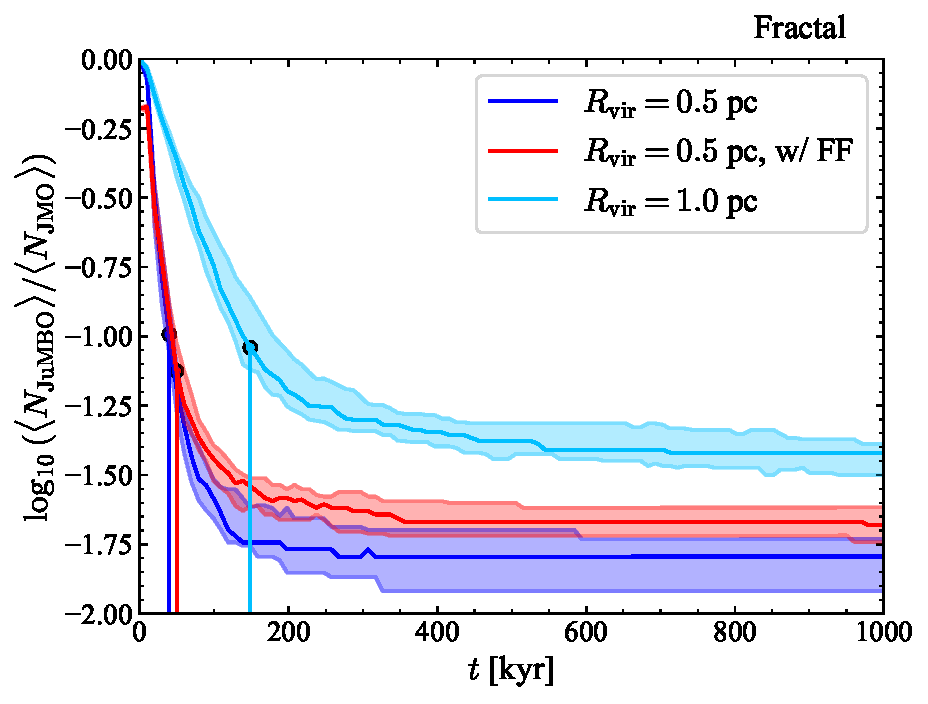
\includegraphics[width=\columnwidth]{figures/Fractal_General__fJuMBO_evol.pdf    }
        \caption{}
         \label{Fig:Fjumbo_vs_time_model_ISF_R05}
   \end{figure}
   
   \begin{figure}
    \centering
        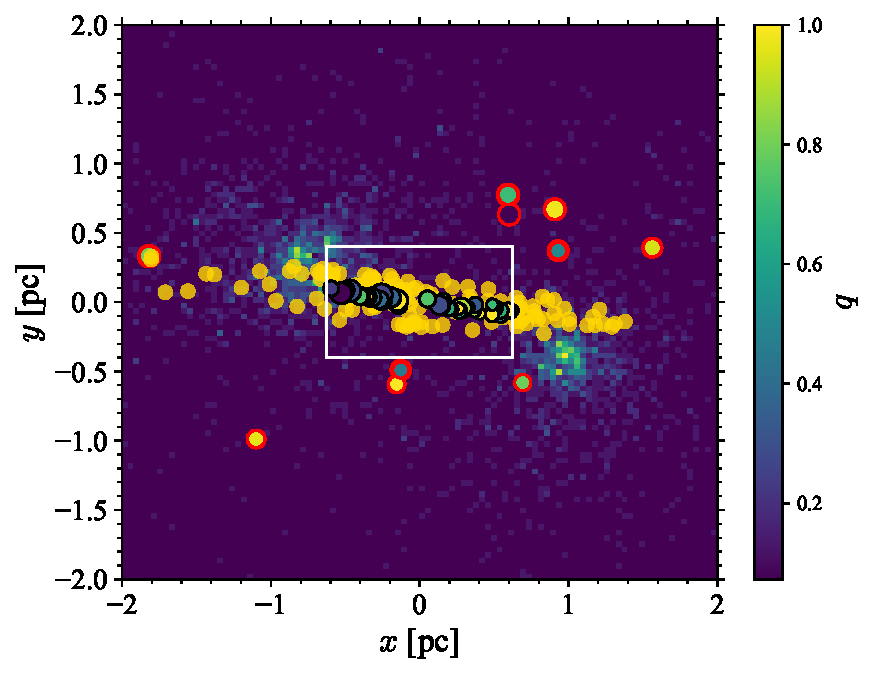
\includegraphics[width=\columnwidth]{figures/overplotting_HEATMAP.pdf}
        \caption{Schematic of a F05 simulation. The density map denotes final positions of simulated objects, the translucent yellow points observed stars taken from \citet{2016A&A...595A...1G, 2023A&A...674A...1G}. The white frame denotes the observed region in \citet{2023arXiv231001231P}, with black outlined dots denoting observed JuMBOs. Red outlined dots denote the final \jumbos\, observed in our simulation.}
         \label{Fig:Overplot}
   \end{figure}

    Figure \ref{Fig:Overplot} shows the final snapshot of a F05 simulation. It represents the typical final state of simulations evolved during our $\mathcal{ISF}$ and $\mathcal{FFC}$ runs. The density map reveals the final positions of all objects simulated. Surviving \jumbos\, are scattered onto the plot with red outlines. Overlayed are also the positions of known stars (in yellow) taken from \citet{2016A&A...595A...1G, 2023A&A...674A...1G} and the positions of known \jumbos\, (black outlined points) \citep{2023arXiv231001231P}.

    Table \ref{Tab:Final_ISF_FFC_Results} summarises all our final results. We begin our discussion on the $\mathcal{ISF}$ models by looking at the general models (top segment of table \ref{Tab:ISF_FFC_Initial}). 
     
    \subsubsection{Open Parameter Space}
    Overall, \jumbos\, are more likely to survive in a Plummer-like cluster. Their survival rates increase by a factor of $\sim 18$ compared with likewise configurations initialised under a Fractal distribution. Even so, no configuration is successful in reproducing the $9\%$ fraction of \jumbos\, relative to free-floaters observed. Instead, in the $\mathcal{ISF}$ scenarios, the fraction of \jumbos\, to JMO free floaters ranges between $0.29\sim1.3$ for Plummer runs and $0.01\sim0.02$ for Fractals.
    
    The increase of \jumbo\, surviveability in runs including free-floaters could be due to the rare JMO-JuMBO interaction hardening the binary, also resulting in a decrease in its gravitational cross section. We believe this to be the case even though as discussed in the introduction \jumbos\, will tend to ionise, even when interacting with other JMO, since, although increasing the number of JMOs enhances the chances of two free-floaters (or a free floater and ionised JMO) settling into a newly formed binary, on average, only $0.4$ new \jumbo\, systems emerge per run for F05 runs compared to the $0.65$ in F05FF (from $1.75$ to $3.15$ between P05 and P05FF). 
    
    Figures \ref{Fig:Gen_Semi_Fractal} show the cumulative distribution function (CDF) for the semi-major axis of surviving \jumbos\, during F05, F05FF and F1 runs. The Fractal distribution efficiently prunes off any wide orbits since its violent nature provokes many encounters result in the ionisation of \jumbo\, systems, moreso the ones on wide orbits who have a larger cross-section. The tendency for \jumbos\, to ionise at any encounter is reflected by the little variation between runs of the same virial radius. We also note the tendency for \jumbos\, to ionise even when a JMO perturbs the system as reflected with the decrease in median semi-major axis between models P05 and P05FF from $\langle a\rangle\sim268$ au to $\langle a\rangle\sim187$ au.
   
   \begin{figure}
    \centering
        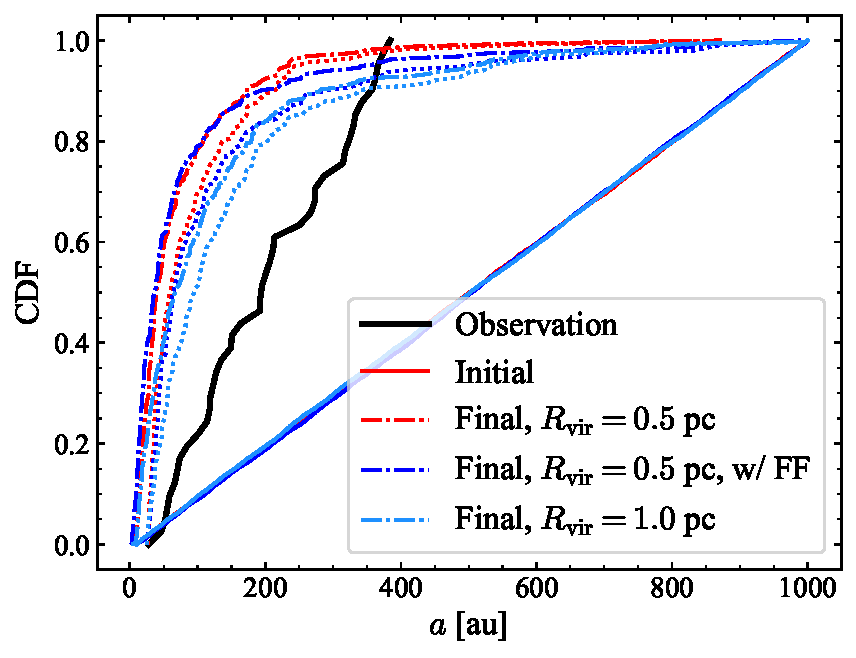
\includegraphics[width=\columnwidth]{figures/Fractal_General_sem_axis.pdf}
        \caption{CDF of surviving \jumbo\, semi-major axis distribution for models F05, F05FF, F1. Dash-dotted curves incorporate all \jumbo\, systems, whereas dotted ones only those with a projected separation exceeding $25$ au.}
         \label{Fig:Gen_Semi_Fractal}
   \end{figure}
    
    The results in semi-major axis' during the Fractal runs are much smaller than those observed, suggesting the $\mathcal{ISF}$ model fails to capture the birth of such environments. Contrariwise, and as seen in figure \ref{Fig:Gen_Semi_Plummer}, Plummer models are capable of preserving the wider orbits. This, however, is due to the environment to output similar values to those inputted since it is less violent by nature.
   
   \begin{figure}
    \centering
        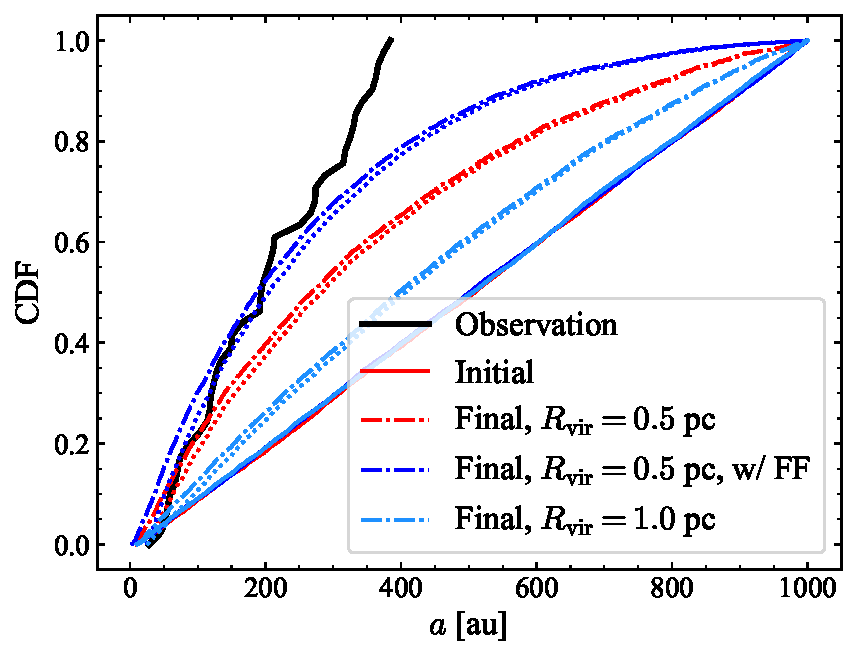
\includegraphics[width=\columnwidth]{figures/Plummer_General_sem_axis.pdf}
        \caption{CDF of surviving \jumbo\, semi-major axis distribution for models P05, P05FF, P1. Dash-dotted curves incorporate all \jumbo\, systems, whereas dotted ones only those with a projected separation exceeding $25$ au.}
         \label{Fig:Gen_Semi_Plummer}
   \end{figure}

    Indeed, keeping in mind that our \jumbos\, in these models are initialised with a uniform mass distribution, we see the uniformity reflected in the final $M_{\mathrm{prim}}$ vs. $q$ parameter space shown in figure \ref{Fig:Gen_mdistr_Plummer}. Although it also fails at reproducing observations, figure \ref{Fig:Gen_mdistr_Fractal} shows more structure and less uniformity in the distribution of \jumbos\, in ($M_{\mathrm{prim}}$, $q$)-space as reflected by the starker contrasts between contour levels and smaller high-density regions.
    
    Given this, although a correct calibration of initial conditions during Plummer runs will give back \jumbos\, with similar properties to those observed, the extent of fine tuning needed and lack of natural mechanism to remove the tail end of wide-orbit JuMBOs, we can apply Occam's razor to rule it out as an initial conditions. 
    
    The omission of Plummer models is further supported since no systems formed dynamically during the runs. This contradicts with the observed presence of two triple JMO systems. Given this, we restrict ourselves to Fractal models as we believe this better represents the Trapezium cluster, a fact agreeing with \citet{2016MNRAS.457..313P}.
   
   \begin{figure}
    \centering
        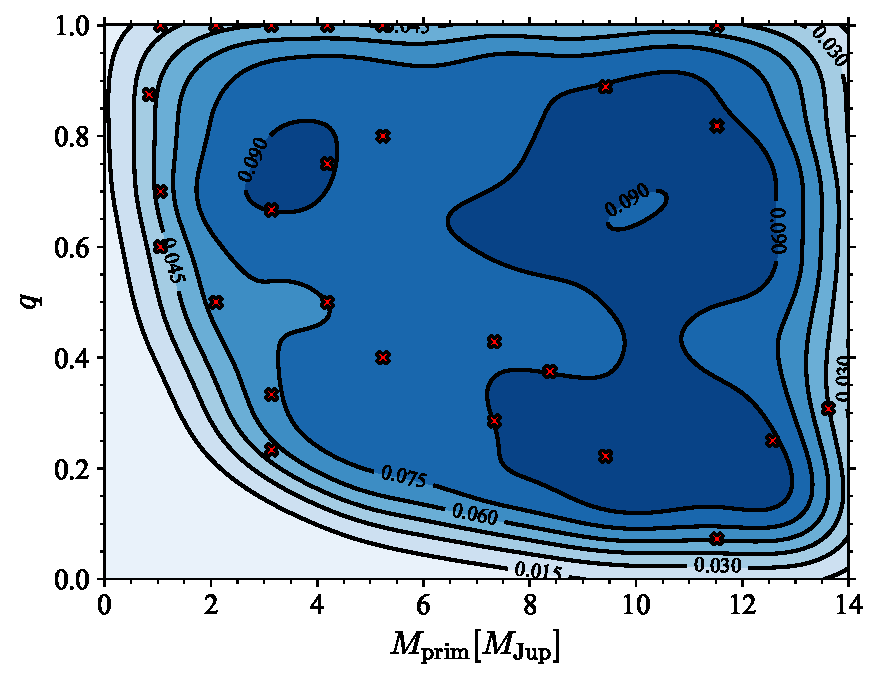
\includegraphics[width=\columnwidth]{figures/Plummer_rvir0.5_FF_mass_distr.pdf}
        \caption{Contour plot of $M_{\mathrm{prim}}$ vs. $q$ for model P05FF. Red crosses denote where observed \jumbos\, lie.}
         \label{Fig:Gen_mdistr_Plummer}
   \end{figure}
   
   \begin{figure}
    \centering
        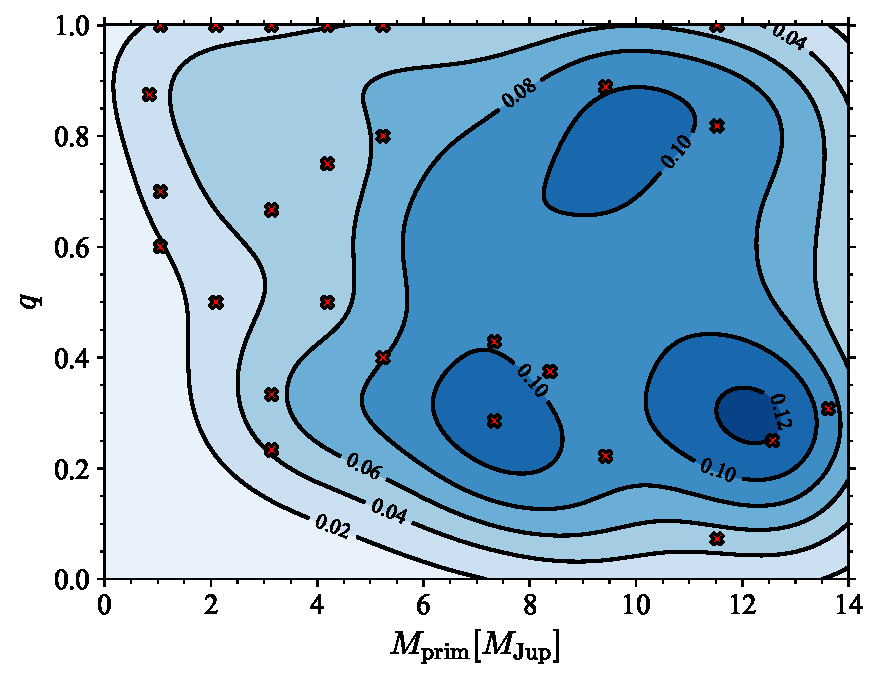
\includegraphics[width=\columnwidth]{figures/Fractal_rvir0.5_FF_mass_distr.pdf}
        \caption{Contour plot of $M_{\mathrm{prim}}$ vs. $q$ for model F05FF. Red crosses denote where observed \jumbos\, lie.}
         \label{Fig:Gen_mdistr_Fractal}
   \end{figure}

    \subsubsection{Evolving till $10$ Myr: TO CHECK -- STILL IN RUNS}
        Here we analyse results for a system evolved to $10$ Myr, with the aim of looking at the survival of \jumbos\, in more established systems. Overall, the \jumbo\, survival rate decreases and the ones surviving exhibit tighter orbits with $\langle a\rangle \sim 20$, a regime in which two $3\ M_{\mathrm{Jup}}$ systems become hard for $\sim M_{\mathrm{Jup}}$ interactions. 
        
        Figure \ref{Fig:Mdistr_SimTime} shows the distribution of $M_{\mathrm{prim}}$ of surviving JuMBOs. The little difference  observed between F05FF and F05FFL is reflected by the similarities between their median and interquartile (IQR) range ($\langle M_{\mathrm{prim}}\rangle\sim 8.8$ and $\langle M_{\mathrm{prim}}\rangle \sim 8.1$ for F05FF and F05FFL respectively). The fact that this holds for all configurations simulated implies the ease at which \jumbo\, systems ionise upon interaction.

        Figure \ref{Fig:SimTime_MPrimQ} shows the contour plot of $M_{\mathrm{prim}}$ vs. $q$. As before, the parameter space poorly replicates the observed distribution with most of the \jumbos\, having too large a primary mass. We keep this in mind for simulations in the following subsection where we initialise \jumbos\, with a power-law of $\alpha = -1.2$, the power-law found to best fit observations.
   
   \begin{figure}
    \centering
        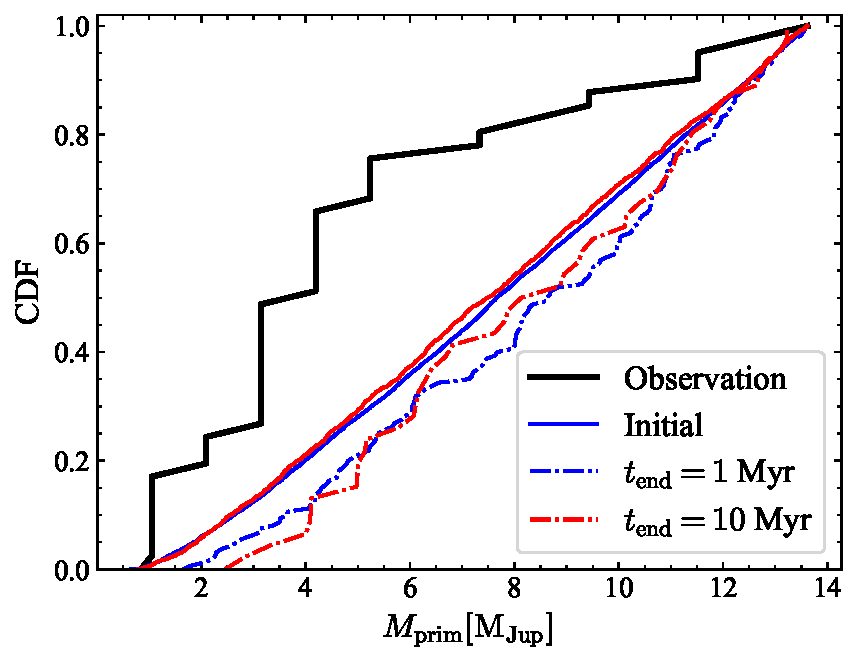
\includegraphics[width=\columnwidth]{figures/SimTime_mprim_vs_obs_.pdf}
        \caption{CDF of surviving \jumbo\, $M_{\mathrm{prim}}$ for models F05FF and F05FFL.}
         \label{Fig:Mdistr_SimTime}
   \end{figure}
   
   \begin{figure}
    \centering
        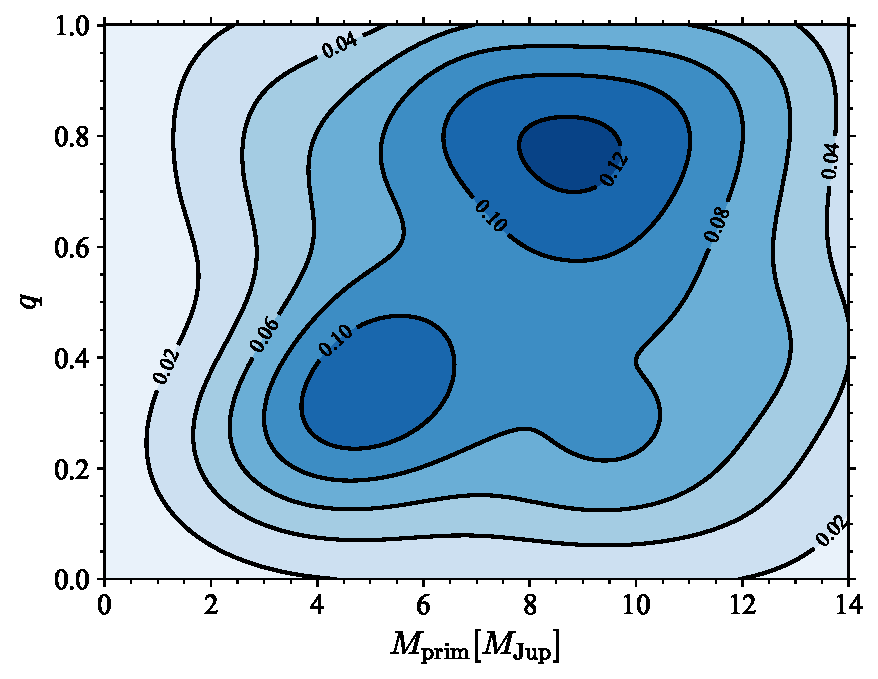
\includegraphics[width=\columnwidth]{figures/Fractal_rvir0.5_FF_10Myr_mass_distr.pdf}
        \caption{$M_{\mathrm{prim}}$ vs. $q$ contour plot for model F05FFL. Red crosses denote where observed \jumbos\, lie.}
         \label{Fig:SimTime_MPrimQ}
   \end{figure}
   
    \subsubsection{Observational Constraints}
    Our preliminary exploration allows us to rule out Plummer models and further constrain the parameter space. When applying these more restricted initial conditions, $f_{\mathrm{surv}}$ and $e$ barely changes while $a$ shows only marginal changes.

    This slight increase in $f_{r_{ij}\geq25\ \mathrm{au}}$, $\langle a\rangle$ and $\langle r_{ij}\rangle$ could be attributed to the reduction of JMO and \jumbos\, present in the environment and the smaller masses they occupy making it harder for them to destabilise wide binaries. The difference in the semi-major axis distribution between models F05, F05O and F05OC (JuMBOs are initially on circular orbits) is shown in figure \ref{Fig:Semi_Fractal}. No matter the configuration, the Fractal models exhibit a natural tendency for trimming out wide binaries.
    
   \begin{figure}
    \centering
        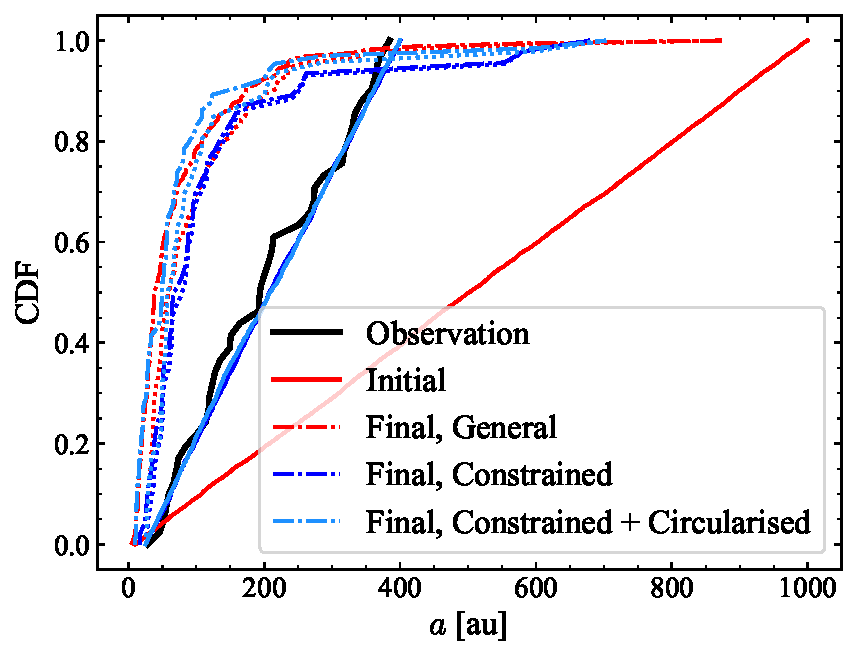
\includegraphics[width=\columnwidth]{figures/Fractal_noFF_sem_axis.pdf}
        \caption{CDF of surviving \jumbo\, semi-major axis distribution for models F05, F05O, F05OC.}
         \label{Fig:Semi_Fractal}
   \end{figure}

   Figure \ref{Fig:Fractal_mdistrCDF} shows the CDF of primary masses comparing models F05, F05O And F05OC. No matter the configuration, a similar evolution is observed where surviving \jumbos\, tend to have larger primary masses. However, unlike the F05 model, the constrained model, initialised with $\alpha = -1.25$, end up being roughly uniform in primary mass compared to the somewhat thermal appearance for F05. In doing, the median primary masses shift towards lower values while the mass ratio towards larger one. A fact reflected by the statistics shown in table \ref{Tab:Final_ISF_FFC_Results} and shown in figure \ref{Fig:FractalObs_mdistr}.
    
   \begin{figure}
    \centering
        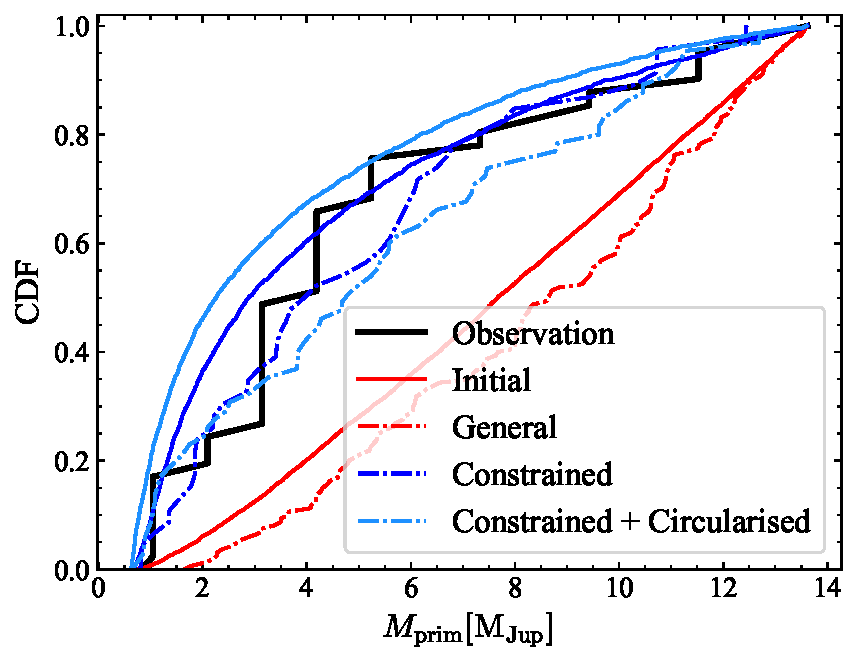
\includegraphics[width=\columnwidth]{figures/Fractal_noFF_mprim_vs_obs_.pdf}
        \caption{CDF of surviving \jumbo\, primary mass for models F05, F05O, F05OC.}
         \label{Fig:Fractal_mdistrCDF}
   \end{figure}

    Over the course of our simulation, Fractal runs exhibit a range of dynamical phenomena. The statistics of merging scenarios, and the emergence of both Jupier-mass - Stellar binary systems and $N\geq3$ systems are summarised in table \ref{Tab:Systems}.

    Jupiter-mass - stellar mergers could ................ In addition to mergers, ejection events also occured. Though no \jumbos\, were ejected, $\sim1$ JMO was ejected per simulation and $\sim 3$ stellar-mass objects.
    
    Figure \ref{Fig:MixedSys_OrbParams} shows where in $(a,e)$-space Jupiter-mass - Stellar binaries lie, with little variation between configurations. The parameter space is widely covered, with signs of low-eccentricity but very wide ($a\geq700$ au) binaries. Nevertheless, the vast majority exhibit large eccentricities and semi-major axis, reflecting their dynamical origin. The non-negligible amount of these systems emerging provide an interesting prospect of detecting ultra-cold Jupiters orbiting stars who have recently fostered them.

    Given the poor reproducability in ratios of \jumbos\, to JMO free floaters and the tight orbits of \jumbos\, we conclude that the $\mathcal{ISF}$ models are most likely not the origins of JuMBOs, lending us to our final possible scenario, $\mathcal{FFC}$.

   \begin{figure}
    \centering
        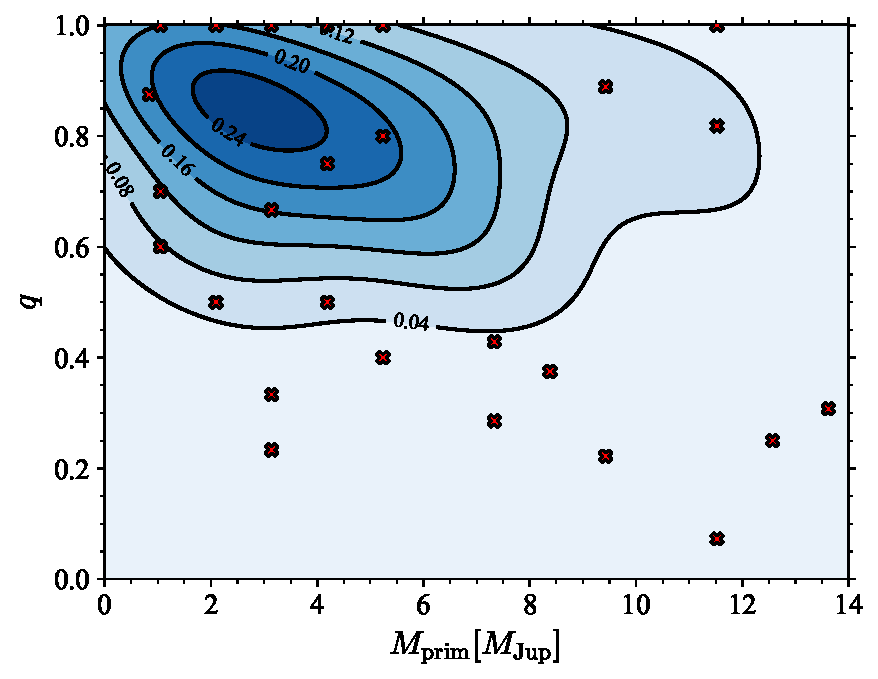
\includegraphics[width=\columnwidth]{figures/Fractal_rvir0.5_Obs_mass_distr.pdf}
        \caption{Contour plot of $M_{\mathrm{prim}}$ vs. $q$ for F05O. Red crosses denote where observed \jumbos\, lie.}
         \label{Fig:FractalObs_mdistr}
   \end{figure}
   
   \begin{figure}
    \centering
        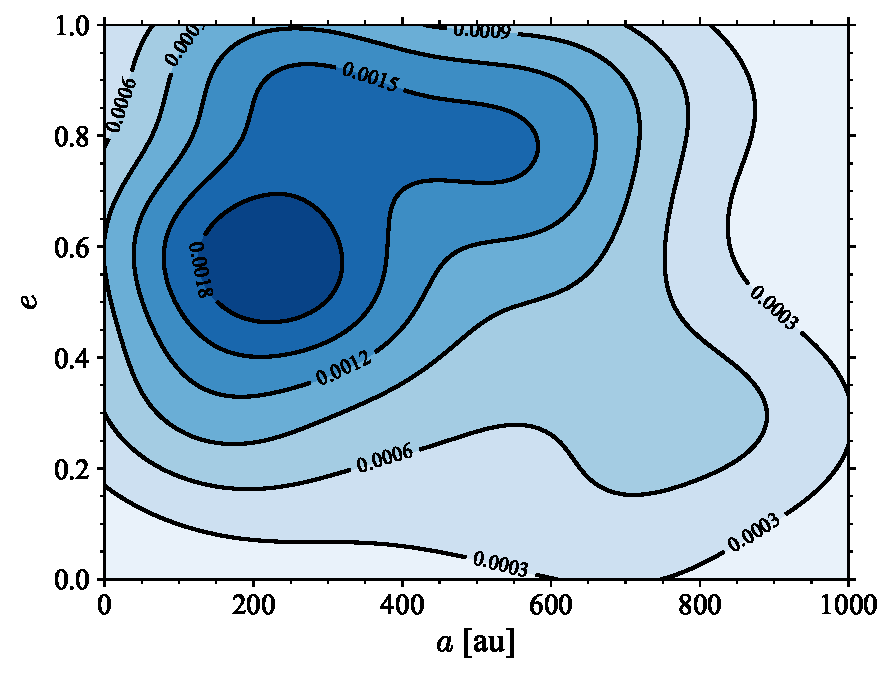
\includegraphics[width=\columnwidth]{figures/Fractal_rvir0.5_FF_Obs_sem_ecc_mixed_systs.pdf}
        \caption{$a$ vs. $e$ parameter space occupied by Star-JMO binaries during F05FFO runs.}
         \label{Fig:MixedSys_OrbParams}
   \end{figure}

    \begin{table}
         \caption{TO CHECK}
        \label{Tab:M2Events} 
        \centering 
        \begin{tabular}{c c c c c}
        \hline\hline
        Model & $\langle N_{\mathrm{JS, merge}}\rangle$ & $\langle N_{\mathrm{SS, merge}}\rangle$ & $\langle N_{\mathrm{JS}}\rangle$ &  $\langle N_{\mathrm{multi}} \rangle$ \\
        \hline \vspace{-0.75em}\\ 
           F05     & $2.5^{+0.5}_{-1.5}$ & $19^{+4}_{-7}$ & $8^{+3}_{-0}$  & $2^{+0}_{-0}$ \vspace{0.25em}\\
           F05FF   & $5.5^{+1.5}_{-1.5}$ & $21^{+2}_{-4}$ & $14^{+1}_{-3}$ & $2^{+0}_{-0}$ \vspace{0.25em}\\
           F1      & $1.0^{+1.0}_{-0.0}$ & $14^{+3}_{-5}$ & $10^{+1}_{-3}$ & $2^{+0}_{-0}$ \vspace{0.25em}\\
           F05FFL  & $5.0^{+0.0}_{-1.0}$ & $22^{+3}_{-5}$ & $1.0^{+0.0}_{-0.0}$ & $0^{+7}_{-0}$ \vspace{0.25em}\\
           \hline \vspace{-0.75em}\\
           F05O    & $2.0^{+0.8}_{-1.8}$ & $25^{+2}_{-8}$ & $4.5^{+2.8}_{-0.5}$ & $2.0^{+0}_{-0}$ \vspace{0.25em}\\
           F05FFO  & $1.0^{+1.0}_{-0.0}$ & $17^{+3}_{-1}$ & $5.0^{+1.5}_{-1.0}$ & $1.0^{+0}_{-0}$ \vspace{0.25em}\\
           F05OC   & $0.5^{+2.3}_{-0.5}$ & $20^{+5}_{-4}$ & $4.5^{+1.5}_{-1.5}$ & $3.5^{+0}_{-0}$ \vspace{0.25em}\\
           \hline
         \hline                               %inserts single line
         \label{Tab:Systems}
        \end{tabular}
     \end{table}
    \subsection{$\mathcal{FFC}$}
    

%--------------------------------------------------------------------
\section{Discussion}
 Lorem ipsum dolor sit amet, consectetur adipiscing elit, sed do eiusmod tempor incididunt ut labore et dolore magna aliqua. Ut enim ad minim veniam, quis nostrud exercitation ullamco laboris nisi ut aliquip ex ea commodo consequat. Duis aute irure dolor in reprehenderit in voluptate velit esse cillum dolore eu fugiat nulla pariatur. Excepteur sint occaecat cupidatat non proident, sunt in culpa qui officia deserunt mollit anim id est laborum.

%--------------------------------------------------------------------

\section{Conclusions}

\subsection{Energy Consumption}
The $820$ simulations conducted during this investigation had a total wall-clock time of $432$ days. For the XYZ runs, each CPU used $6$ cores, for the other two configurations $18$ cores were used per CPU. In total, the CPU time for all simulations was $7680$ days. Assuming a CPU consumption rate of $12$ Watt hr$^{-1}$ \citep{PortegiesZwart2020}, the total energy consumption is roughly $2210$ kWh. For an emission intensity of $0.283$ kWh kg$^{-1}$ \citep{Wittman}, our calculations emitted $7.8$ tonnes of CO2, roughly equivalent to two round trips by plane New York - Beijing.

\begin{acknowledgements}
Veronica  Saz  Ulibarrena,  Shuo  Huang,  Maite  Wilhelm,  Brent Maas
\end{acknowledgements}

% for the bibliography, at the end
\bibliographystyle{aa} % style aa.bst
\bibliography{references.bib} % your references Yourfile.bib

\begin{appendix}
    \section{Similarity between $r_{ij}$ and $a$}
    Figures \ref{Fig:Plummer_rsep} and \ref{Fig:Fractal_rsep} motivate our choice of analysing results in terms of the semi-major axis given the similarity between the curves. 
    
    In all cases, $r_{ij}$ exhibits longer tails at the detriment of the shorter separations/orbits. However, these differences are so small - especially in the Fractal case for which most of our discussion revolves around - that we can safely interchange between one and the other. In doing so, we assume that the observed projected separation of \jumbos\, are equivalent to their semi-major axis, easing our discussion.
    
    \begin{figure}
    \centering
        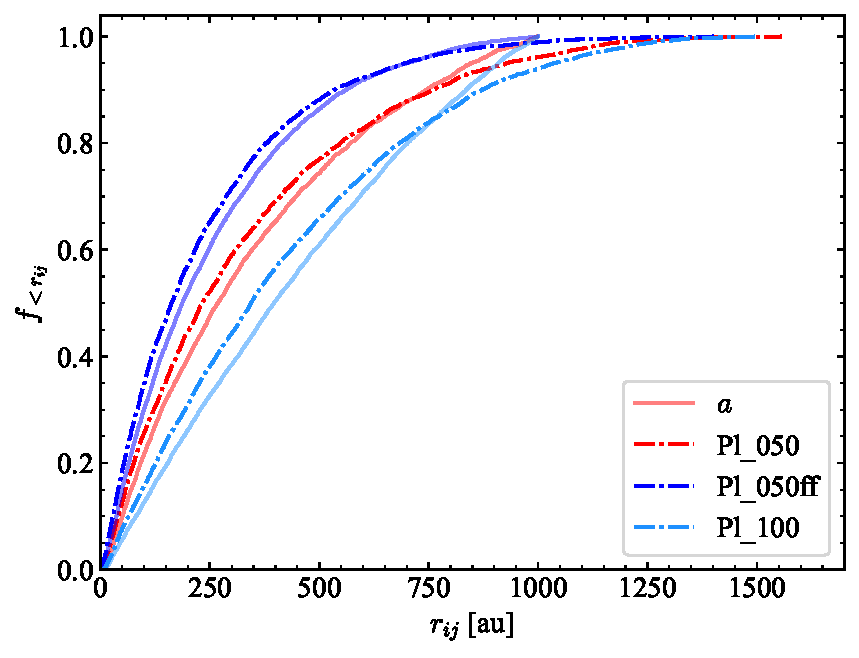
\includegraphics[width=\columnwidth]{figures/Plummer_General_proj_sep.pdf}
        \caption{CDF of surviving \jumbo\, projected separation distribution for models P05, P05FF, P1. Overplotted are translucent lines denoting the respective models' \jumbos\, semi-major axis.}
         \label{Fig:Plummer_rsep}
   \end{figure}
   \begin{figure}
    \centering
        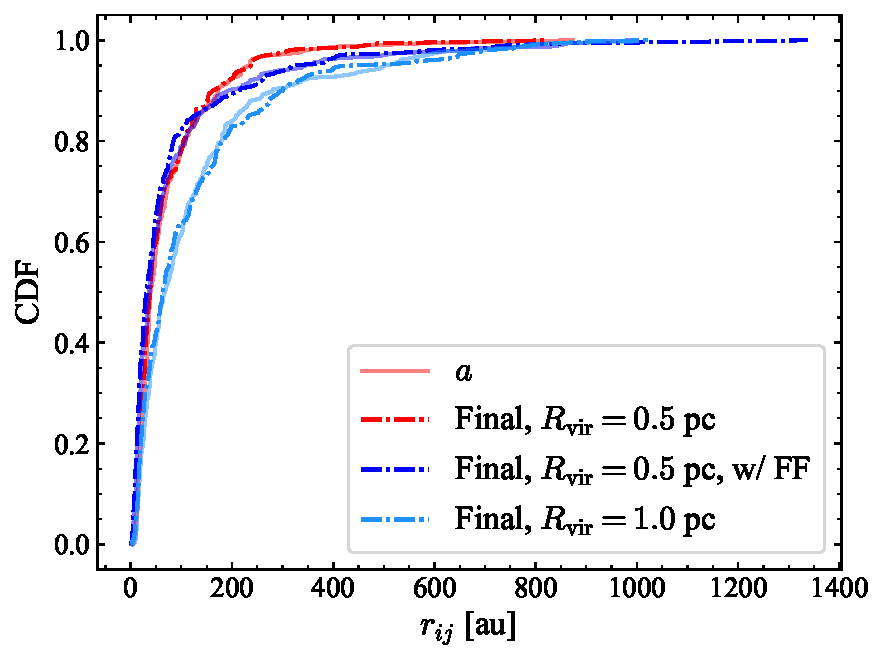
\includegraphics[width=\columnwidth]{figures/Fractal_General_proj_sep.pdf}
        \caption{CDF of surviving \jumbo\, projected separation distribution for models F05, F05FF, F1. Overplotted are translucent lines denoting the respective models' \jumbos\, semi-major axis.}
         \label{Fig:Fractal_rsep}
   \end{figure}
\end{appendix}


\section*{Acknowledgements}

Veronica Saz Ulibarrena, Shuo Huang, Maite Wilhelm, Brent Maas,
Fred Rasio, Alvaro Hacar.
    
\input /home/spz/Latex/lib/bib/references
    
\end{document}

%%%%%%%%%%%%%%%%%%%%%%%%%%%%%%%%%%%%%%%%%%%%%%%%%%%%%%%%%%%%%%
%-------------------------------------------------------------------
% END OF TEXT
%-------------------------------------------------------------------
%%%%%%%%%%%%%%%%%%%%%%%%%%%%%%%%%%%%%%%%%%%%%%%%%%%%%%%%%%%%%%

Pl
Rvir N/run <M>	<m>	<a>	<e>	Nruns
0.25 0.4   7.35	2.35	2388	0.70	40
0.50 0.7   6.76	2.44	2196	0.86	10
1.00 0.4   3.77	1.67	1507	0.28	10

Fr1.6 
Rvir N/run <M>	<m>	<a>	<e>	Nruns
0.25 0.0				10
0.50 0.1   3.8	1.9	118	0.99	10
1.00 0.2   8.3	5.8	147	0.94	10

Pl with Rvir= 0.25pc with various secondary planet orbits (rHill)
rH N/run <M>	<m>	<a>	<e>	Nruns
10 0.4   7.35	2.35	2388	0.70	40
5  2.6	 8.32	2.27	1895	0.78	10
2  8.6	 6.60	2.89	1448	0.82	10

Pl with Rvir= 0.25pc at various times (t)
t   N/run  <M>	<m>	<a>	<e>	Nruns
1.0 0.40   7.35	2.35	2388	0.70	40
0.5 0.15   5.43	1.58	4400	0.67	40

Pl with Rvir= 0.25pc rH=5, q=sqrt() 
t   N/run  <M>	<m>	<a>	<e>	Nruns
1.0 0.8	   2.50 1.36   2716.31   0.777  10

SPP models:
F,amin,amax,Nbs,Nbp,Nss,Nsp,Npp,    M,dM,m,dm,q,dq,a,da,e,de
PlN2500n600cs_R0.25pcQ05_R.0010.csv,0,1,87.9,0.15,0.0,197.575,0.75,   1.5182175287307713,0.560698545375267,4.214078182297578,4.095751989095275,2.3313106716943386,1.6790659126026926,496.95907830935147,281.2222075471759,0.8733079229200573,0.09833531990765235
PlN2500n600cs_R0.5pcQ05_R.0010.csv,0,1,88.9,0.3,0.0,201.3,1.0    ,nan,nan,nan,nan,nan,nan,nan,nan,nan,nan
PlN2500n600cs_R1.0pcQ05_R.0010.csv,0,1,85.8,0.1,0.0,195.2,0.8,3.270505088406785,    0.0,1.316197735754376,0.0,0.4024447906899778,0.0,673.1443537047858,0.0,0.08404250840976944,0.0

FrN2500n600cs_R0.25pcQ05_R.0011.csv,0,1,13.399999999999999,0.0,71.3,43.6,0.1,nan,nan,nan,nan,nan,nan,nan,nan,nan,nan



SPM models:

F,amin,amax,Nbs,Nbp,Nss,Nsp,Npp,M,dM,m,dm,q,dq,a,da,e,de
PlN2500n600pm_R0.5pcQ05_R.0010.csv,0,1,51.2,50.7,0.0,61.3,567.1,3.241863236847126,3.146419649374478,4.1994324138885455,3.6477551651523243,2.292947966246368,2.9219855055516857,224.8664798090486,107.62369768018677,0.21362638856650273,0.24988436693392485

F,amin,amax,Nbs,Nbp,Nss,Nsp,Npp,M,dM,m,dm,q,dq,a,da,e,de
FrN2500n600pm_R0.5pcQ05_R.0011.csv,0,1,6.0,1.9,68.6,15.8,103.1,3.5484148732876206,3.317421904592993,4.905084847828215,4.019173763984519,2.5668243481935926,3.2345942681146256,175.82553098470015,150.19026253990216,0.4658461018866108,0.2849317239089184
F,amin,amax,Nbs,Nbp,Nss,Nsp,Npp,    M,dM,m,dm,q,dq,a,da,e,de
PlN2500n600cs_R0.25pcQ05_R.0010.csv,0,1,87.9,0.15,0.0,197.575,0.75,   1.5182175287307713,0.560698545375267,4.214078182297578,4.095751989095275,2.3313106716943386,1.6790659126026926,496.95907830935147,281.2222075471759,0.8733079229200573,0.09833531990765235
PlN2500n600cs_R0.5pcQ05_R.0010.csv,0,1,88.9,0.3,0.0,201.3,1.0    ,nan,nan,nan,nan,nan,nan,nan,nan,nan,nan
PlN2500n600cs_R1.0pcQ05_R.0010.csv,0,1,85.8,0.1,0.0,195.2,0.8,3.270505088406785,    0.0,1.316197735754376,0.0,0.4024447906899778,0.0,673.1443537047858,0.0,0.08404250840976944,0.0

